\documentclass[10pt,xcolor={dvipsnames}]{beamer}

\usepackage{amsmath}
\usepackage{amssymb}
\usepackage{graphicx}
%\usepackage{framed}
\usepackage[american]{circuitikz}
%\usepackage{pgfplots}
\usetikzlibrary{arrows.meta,overlay-beamer-styles,positioning,calc,fit}
%\usepackage[american]{circuitikz}
\usepackage{siunitx}
\usepackage[T1]{fontenc}
\usepackage{subcaption}
%\usepackage{mathtools}
%\usepackage{makecell}
%\usepackage{steinmetz}
%\usepackage{calc}

% set default graphics path to ``figs''
\graphicspath{{figs}}

\beamertemplatenavigationsymbolsempty
\setbeamertemplate{footline}{%
	\raisebox{10pt}{\makebox[\paperwidth]{\hfill\makebox[30pt]{\scriptsize\insertframenumber}}}}

%\pgfplotsset{compat=newest}
%\tikzset{>=Stealth}
%\pgfplotsset{
%	standard/.style={
%		trig format=rad,
%		axis x line=middle,
%		axis y line=middle,
%		enlarge x limits=0.15,
%		enlarge y limits=0.15,
%		x label style={right},
%		y label style={above},
%		y tick label style={right},
%		axis line style={-Stealth,semithick},
%		major tick style={thick,black},
%		extra x tick labels={\empty},
%		extra y tick labels={\empty}
%	}
%}
\let\union\cup
\let\intersect\cap
\let\w\omega
\let\e\epsilon
\let\ve\varepsilon
\let\prefto\succ
\let\nprefto\prec
\let\ans\tcboxmath

\let\Re\relax
\DeclareMathOperator{\Re}{Re}
\let\Im\relax
\DeclareMathOperator{\Im}{Im}
\DeclareMathOperator{\Nul}{Nul}
\DeclareMathOperator{\Col}{Col}
\DeclareMathOperator{\Row}{Row}
\DeclareMathOperator{\Span}{Span}
\DeclareMathOperator{\tr}{tr}
\DeclareMathOperator{\rref}{rref}

\newcommand{\V}[1]{V_{\text{#1}}}
\newcommand{\VR}[1]{V_{R_{\text{#1}}}}
\newcommand{\VL}[1]{V_{L_{\text{#1}}}}
\newcommand{\VC}[1]{V_{C_{\text{#1}}}}
\newcommand{\Vv}[1]{v_{\text{#1}}}

\newcommand{\I}[1]{I_{\text{#1}}}
\newcommand{\IR}[1]{I_{R_{\text{#1}}}}
\newcommand{\IL}[1]{I_{L_{\text{#1}}}}
\newcommand{\IC}[1]{I_{C_{\text{#1}}}}
\newcommand{\Ii}[1]{i_{\text{#1}}}

\renewcommand{\P}[1]{P_{\text{#1}}}
\newcommand{\PR}[1]{P_{R_{\text{#1}}}}
\newcommand{\PL}[1]{P_{L_{\text{#1}}}}
\newcommand{\PC}[1]{P_{C_{\text{#1}}}}

\newcommand{\U}[1]{U_{\text{#1}}}
\newcommand{\E}[1]{E_{\text{#1}}}

\newcommand{\A}[1]{A_{\text{#1}}}

\newcommand{\Z}[1]{Z_{\text{#1}}}
\newcommand{\R}[1]{R_{\text{#1}}}
\newcommand{\Rr}[1]{r_{\text{#1}}}
\newcommand{\C}[1]{C_{\text{#1}}}
\newcommand{\Ll}[1]{L_{\text{#1}}}

\newcommand{\qv}[1]{\qty{#1}{\volt}}
\newcommand{\qkv}[1]{\qty{#1}{\kilo\volt}}
\newcommand{\qmv}[1]{\qty{#1}{\milli\volt}}
\newcommand{\quv}[1]{\qty{#1}{\micro\volt}}
\newcommand{\qnv}[1]{\qty{#1}{\nano\volt}}
\newcommand{\qMv}[1]{\qty{#1}{\mega\volt}}

\newcommand{\qa}[1]{\qty{#1}{\ampere}}
\newcommand{\qma}[1]{\qty{#1}{\milli\ampere}}
\newcommand{\qua}[1]{\qty{#1}{\micro\ampere}}
\newcommand{\qna}[1]{\qty{#1}{\nano\ampere}}

\newcommand{\qw}[1]{\qty{#1}{\watt}}
\newcommand{\qkw}[1]{\qty{#1}{\kilo\watt}}
\newcommand{\qmw}[1]{\qty{#1}{\milli\watt}}
\newcommand{\quw}[1]{\qty{#1}{\micro\watt}}
\newcommand{\qnw}[1]{\qty{#1}{\nano\watt}}
\newcommand{\qMw}[1]{\qty{#1}{\mega\watt}}

\newcommand{\qj}[1]{\qty{#1}{\joule}}
\newcommand{\qkj}[1]{\qty{#1}{\kilo\joule}}
\newcommand{\qmj}[1]{\qty{#1}{\milli\joule}}
\newcommand{\quj}[1]{\qty{#1}{\micro\joule}}
\newcommand{\qnj}[1]{\qty{#1}{\nano\joule}}
\newcommand{\qMj}[1]{\qty{#1}{\mega\joule}}

\newcommand{\qr}[1]{\qty{#1}{\ohm}}
\newcommand{\qkr}[1]{\qty{#1}{\kilo\ohm}}
\newcommand{\qmr}[1]{\qty{#1}{\milli\ohm}}
\newcommand{\qur}[1]{\qty{#1}{\micro\ohm}}
\newcommand{\qnr}[1]{\qty{#1}{\nano\ohm}}
\newcommand{\qMr}[1]{\qty{#1}{\mega\ohm}}

\newcommand{\qf}[1]{\qty{#1}{\farad}}
\newcommand{\qmf}[1]{\qty{#1}{\milli\farad}}
\newcommand{\quf}[1]{\qty{#1}{\micro\farad}}
\newcommand{\qnf}[1]{\qty{#1}{\nano\farad}}
\newcommand{\qpf}[1]{\qty{#1}{\pico\farad}}

\newcommand{\qh}[1]{\qty{#1}{\henry}}
\newcommand{\qmh}[1]{\qty{#1}{\milli\henry}}
\newcommand{\quh}[1]{\qty{#1}{\micro\henry}}
\newcommand{\qnh}[1]{\qty{#1}{\nano\henry}}

\newcommand{\qhz}[1]{\qty{#1}{\hertz}}
\newcommand{\qkhz}[1]{\qty{#1}{\kilo\hertz}}
\newcommand{\qMhz}[1]{\qty{#1}{\mega\hertz}}
\newcommand{\qGhz}[1]{\qty{#1}{\giga\hertz}}
\newcommand{\qThz}[1]{\qty{#1}{\tera\hertz}}

\newcommand{\qkm}[1]{\qty{#1}{\kilo\meter}}
\newcommand{\qm}[1]{\qty{#1}{\meter}}
\newcommand{\qcm}[1]{\qty{#1}{\centi\meter}}
\newcommand{\qmm}[1]{\qty{#1}{\milli\meter}}
\newcommand{\qum}[1]{\qty{#1}{\micro\meter}}
\newcommand{\qnm}[1]{\qty{#1}{\nano\meter}}
\newcommand{\qpm}[1]{\qty{#1}{\pico\meter}}

\newcommand{\qkg}[1]{\qty{#1}{\kilo\gram}}
\newcommand{\qg}[1]{\qty{#1}{\gram}}
\newcommand{\qmg}[1]{\qty{#1}{\milli\gram}}
\newcommand{\qug}[1]{\qty{#1}{\micro\gram}}

\newcommand{\qs}[1]{\qty{#1}{\second}}
\newcommand{\qms}[1]{\qty{#1}{\milli\second}}
\newcommand{\qus}[1]{\qty{#1}{\micro\second}}
\newcommand{\qns}[1]{\qty{#1}{\nano\second}}
\newcommand{\qps}[1]{\qty{#1}{\pico\second}}

\newcommand{\qnc}[1]{\qty{#1}{\nano\coulomb}}

\newcommand{\qdb}[1]{\qty{#1}{\decibel}}
\title{FOC Motor Controller for Drones}
\author{Erk Sampat}
\date{October 3, 2025}
\begin{document}
\begin{frame}
	\begin{center}
		
\includegraphics[height=0.75in]{logo}
	\end{center}
	\vskip-0.5in
	\titlepage
\end{frame}
\begin{frame}\frametitle{Outline}
	\begin{enumerate}
		\item Project Introduction
		\item Theory
		\item Design Walkthrough
	\end{enumerate}
\end{frame}
\begin{frame}\frametitle{Project Introduction -- The Problem}
	\begin{itemize}
		\item Typical FPV drone flight time: 5--7 minutes
		\item Off-the-shelf brushless motor controller efficiency $\approx 70\%$
		\item Can we achieve closer to $100\%$?
		\item Yes! With a better control scheme.
		\item Motor controller (``ESC'') is accessible for improvement
	\end{itemize}
	\begin{center}
		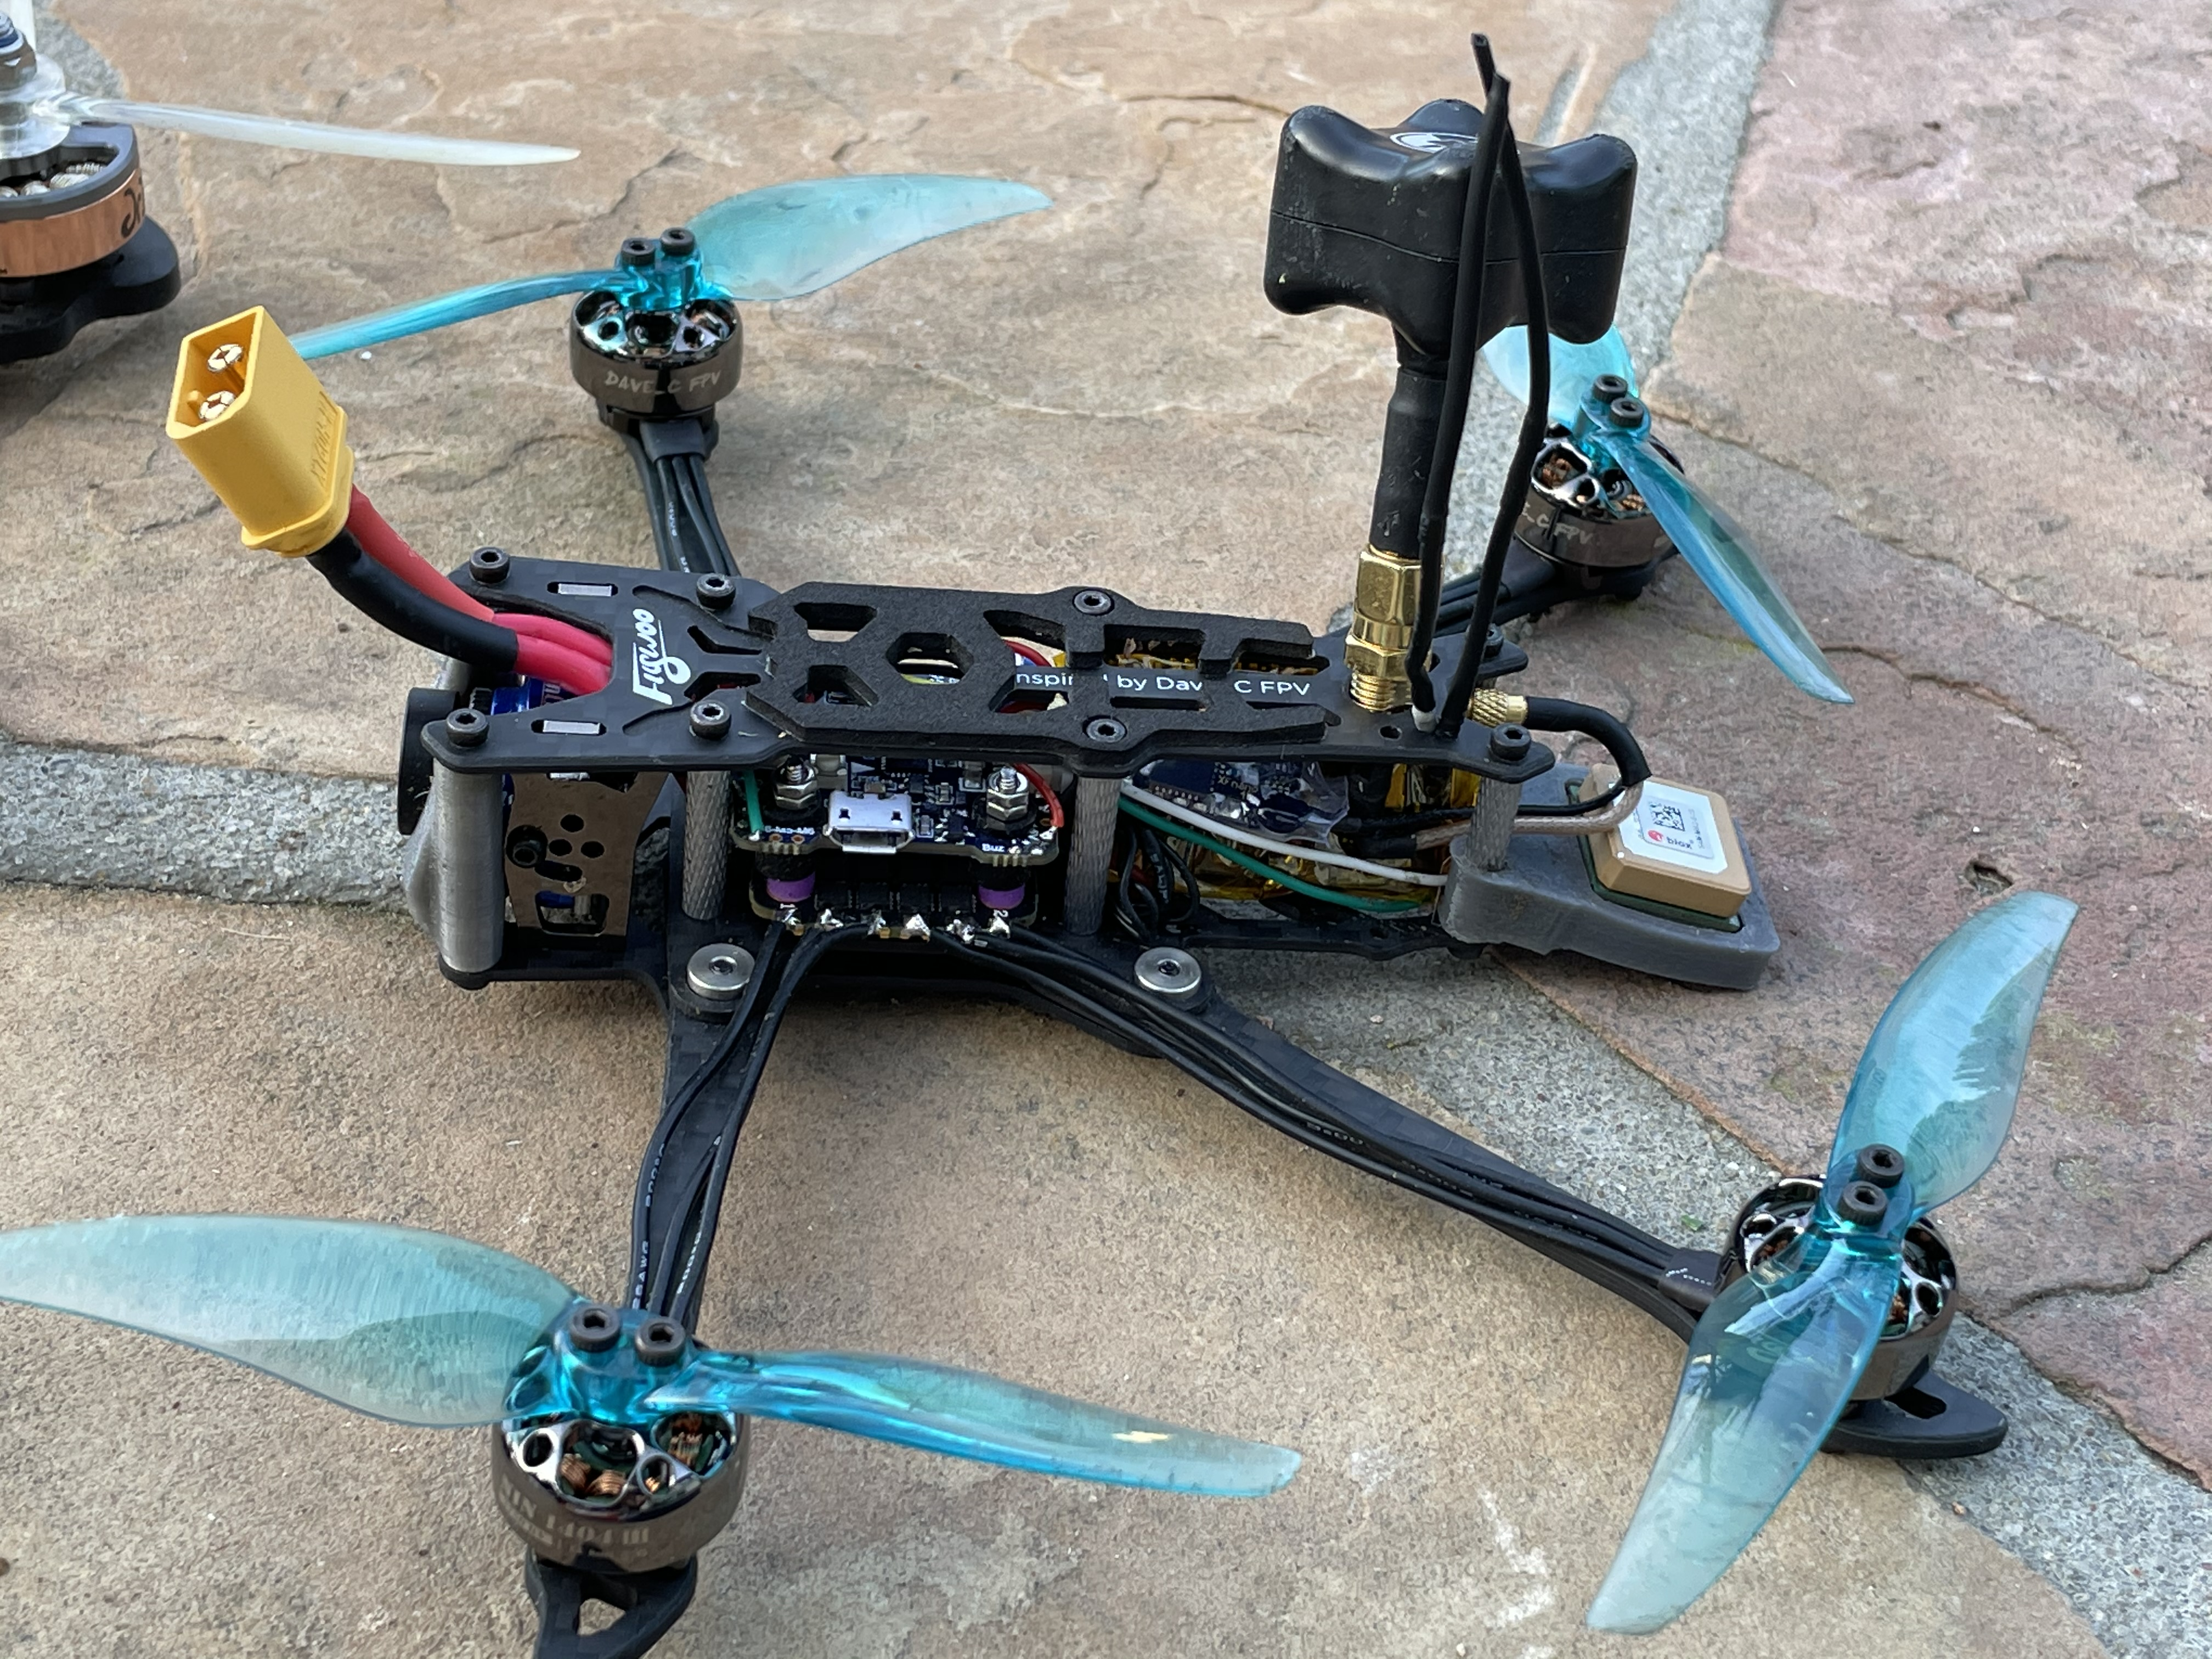
\includegraphics[width=0.6\textwidth]{drone}
	\end{center}
\end{frame}
\begin{frame}\frametitle{Project Introduction -- System Overview}
	\only<1-2>{
		\begin{center}
			\begin{tikzpicture}[scale=0.9,transform shape]
	% Paths, nodes and wires:
	\node[shape=rectangle, draw, line width=0.5pt, minimum width=5.982cm, minimum height=4.982cm] at (35, -4){};
	\node[shape=rectangle, draw, line width=0.5pt, minimum width=2.232cm, minimum height=0.982cm] at (35, -0.75){} node[anchor=center, align=center, text width=1.862cm, inner sep=5.5pt] at (35, -0.75){Battery};
	\node[shape=rectangle, draw, line width=0.5pt, minimum width=2.232cm, minimum height=0.982cm] at (30.625, -4){} node[anchor=center, align=center, text width=1.862cm, inner sep=5.5pt] at (30.625, -4){RC Receiver};
	\node[shape=rectangle, draw, line width=0.5pt, dash pattern={on 2pt off 1pt}, minimum width=2.482cm, minimum height=0.982cm] at (35, -5.5){} node[anchor=center, align=center, text width=2.112cm, inner sep=5.5pt] at (35, -5.5){IMU};
	\node[shape=rectangle, draw, line width=0.5pt, dash pattern={on 2pt off 1pt}, minimum width=2.482cm, minimum height=0.982cm] at (35, -4){} node[anchor=center, align=center, text width=2.112cm, inner sep=5.5pt] at (35, -4){MCU};
	\node[shape=rectangle, draw, line width=0.5pt, dash pattern={on 2pt off 1pt}, minimum width=2.482cm, minimum height=0.982cm] at (35, -2.5){} node[anchor=center, align=center, text width=2.112cm, inner sep=5.5pt] at (35, -2.5){Power Distribution};
	\path[draw=Red, line width=0.8pt, -latex] (35, -1.25) -- (35, -2);
	\draw[-latex] (31.75, -4) -- (33.75, -4);
	\draw[-latex] (35, -5) -- (35, -4.5);
	\path[draw=Red, line width=0.8pt, -latex] (36.75, -2.5) -- (36.75, -5.5) -- (36.25, -5.5);
	\node[shape=rectangle, minimum width=3.215cm, minimum height=0.965cm] at (33.375, -1.75){} node[anchor=center, align=center, text width=2.827cm, inner sep=6pt] at (33.375, -1.75){Flight Controller};
	\only<1>{\node[shape=rectangle, draw, line width=0.5pt, minimum width=2.215cm, minimum height=0.965cm] at (39.375, -4){} node[anchor=center, align=center, text width=1.827cm, inner sep=6pt] at (39.375, -4){4x ESC};}
	\only<2>{\node[shape=rectangle, draw=blue, line width=1pt, minimum width=2.215cm, minimum height=0.965cm] at (39.375, -4){} node[anchor=center, align=center, text width=1.827cm, inner sep=6pt] at (39.375, -4){4x ESC};}
	\node[shape=rectangle, draw, line width=0.5pt, minimum width=2.232cm, minimum height=0.982cm] at (39.375, -5.5){} node[anchor=center, align=center, text width=1.862cm, inner sep=5.5pt] at (39.375, -5.5){4x Motor};
	\path[draw=Red, line width=0.8pt, -latex] (36.75, -4.25) -- (36.25, -4.25);
	\draw[-latex] (35, -3) -- (35, -3.5);
	\path[draw=Red, line width=0.8pt, latex-] (30.625, -3.5) |- (30.75, -2.5) -- (33.75, -2.5);
	\path[draw=Red, line width=0.8pt, -latex] (36.25, -2.5) -| (39.375, -3.5);
	\draw[-latex] (36.25, -4) -- (38.25, -4);
	\path[draw=Red, line width=0.8pt, -latex] (39.375, -4.5) -- (39.375, -5);
\end{tikzpicture}
		\end{center}
	}
	\only<3>{
		\begin{center}
			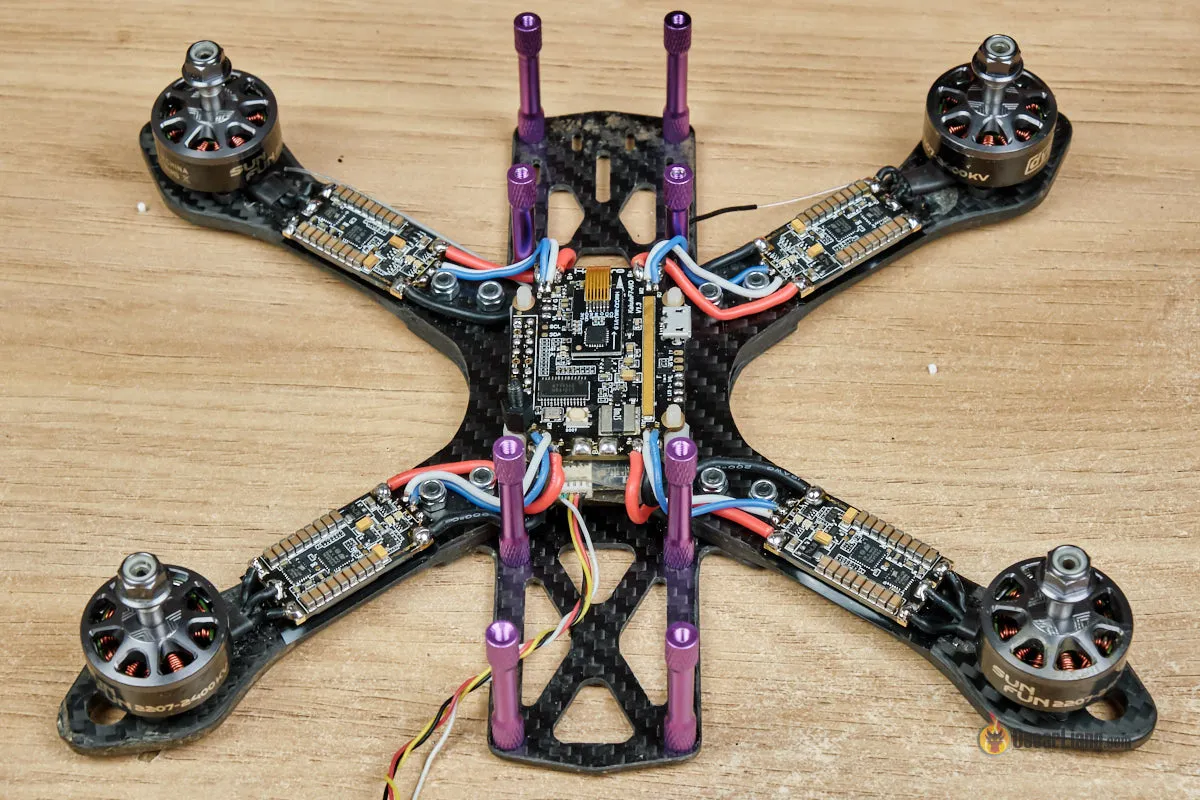
\includegraphics[height=0.45\textheight]{esc_mounted}
			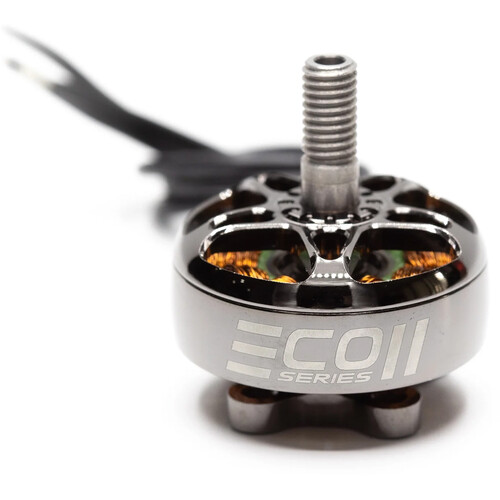
\includegraphics[height=0.45\textheight]{motor}
		\end{center}
	}
\end{frame}
\begin{frame}\frametitle{Project Introduction -- Scope}
	\begin{itemize}
		\item Designed/fabricated/tested custom hardware to run sensorless FOC
		\item Hardware initially designed in 2020
		\item Future plan: fully custom firmware
	\end{itemize}
	\begin{center}
		\only<1>{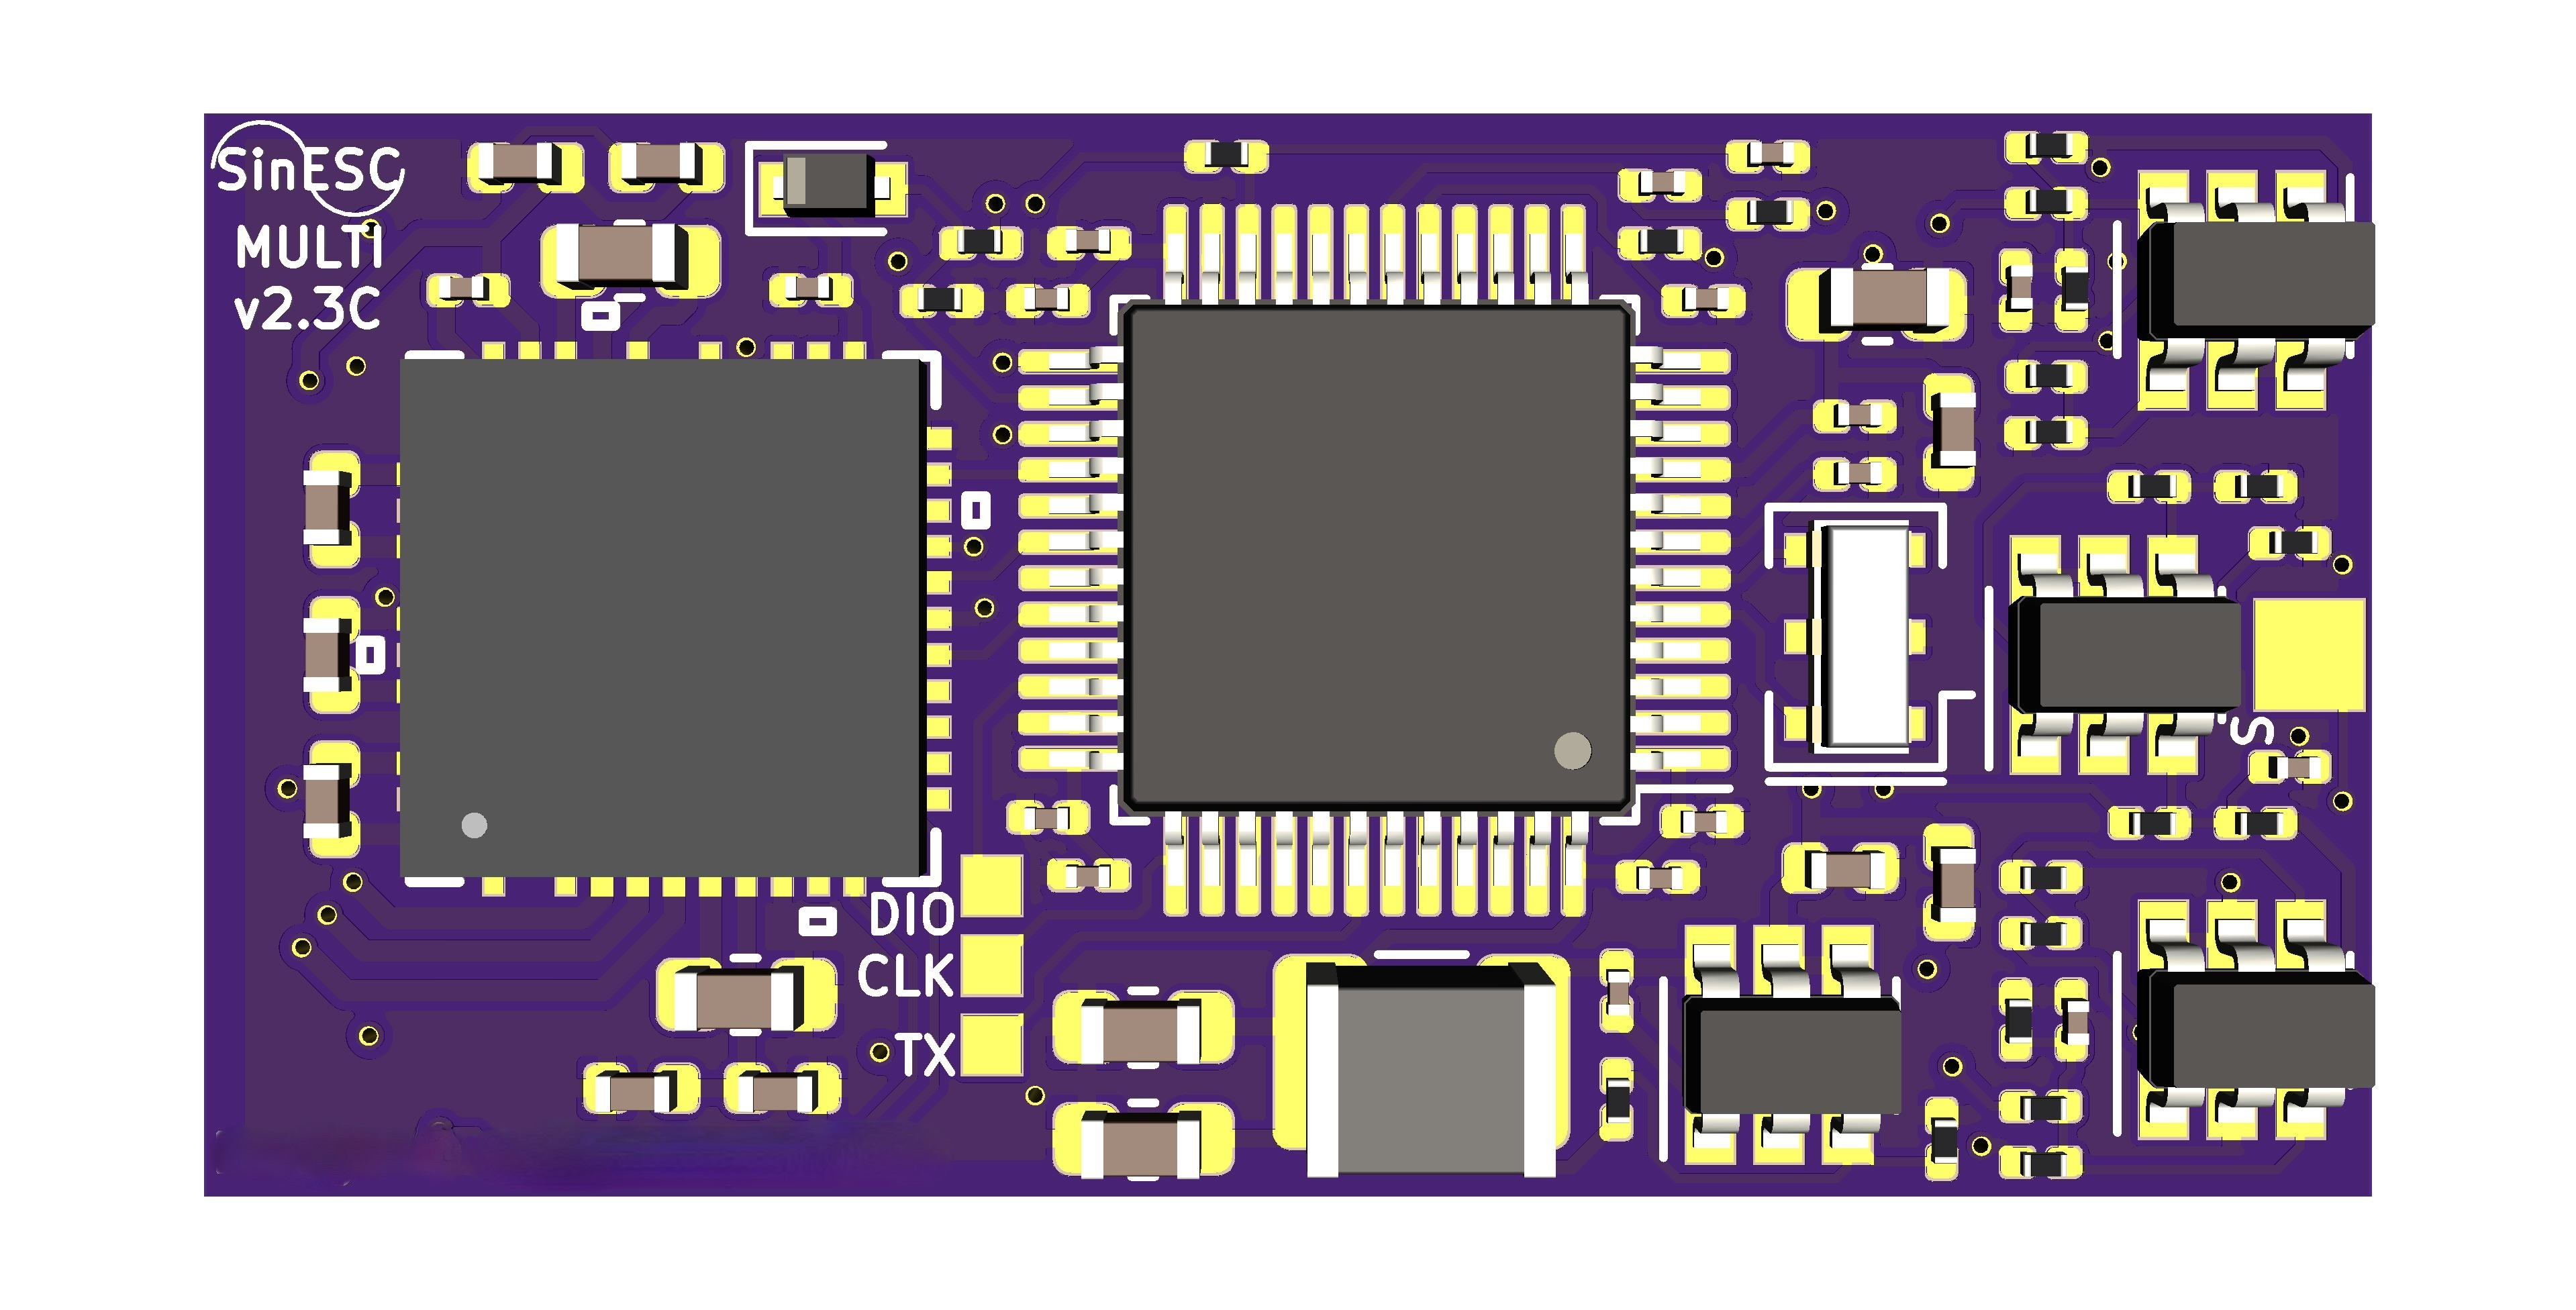
\includegraphics[width=\textwidth]{esc_front}}
		\only<2>{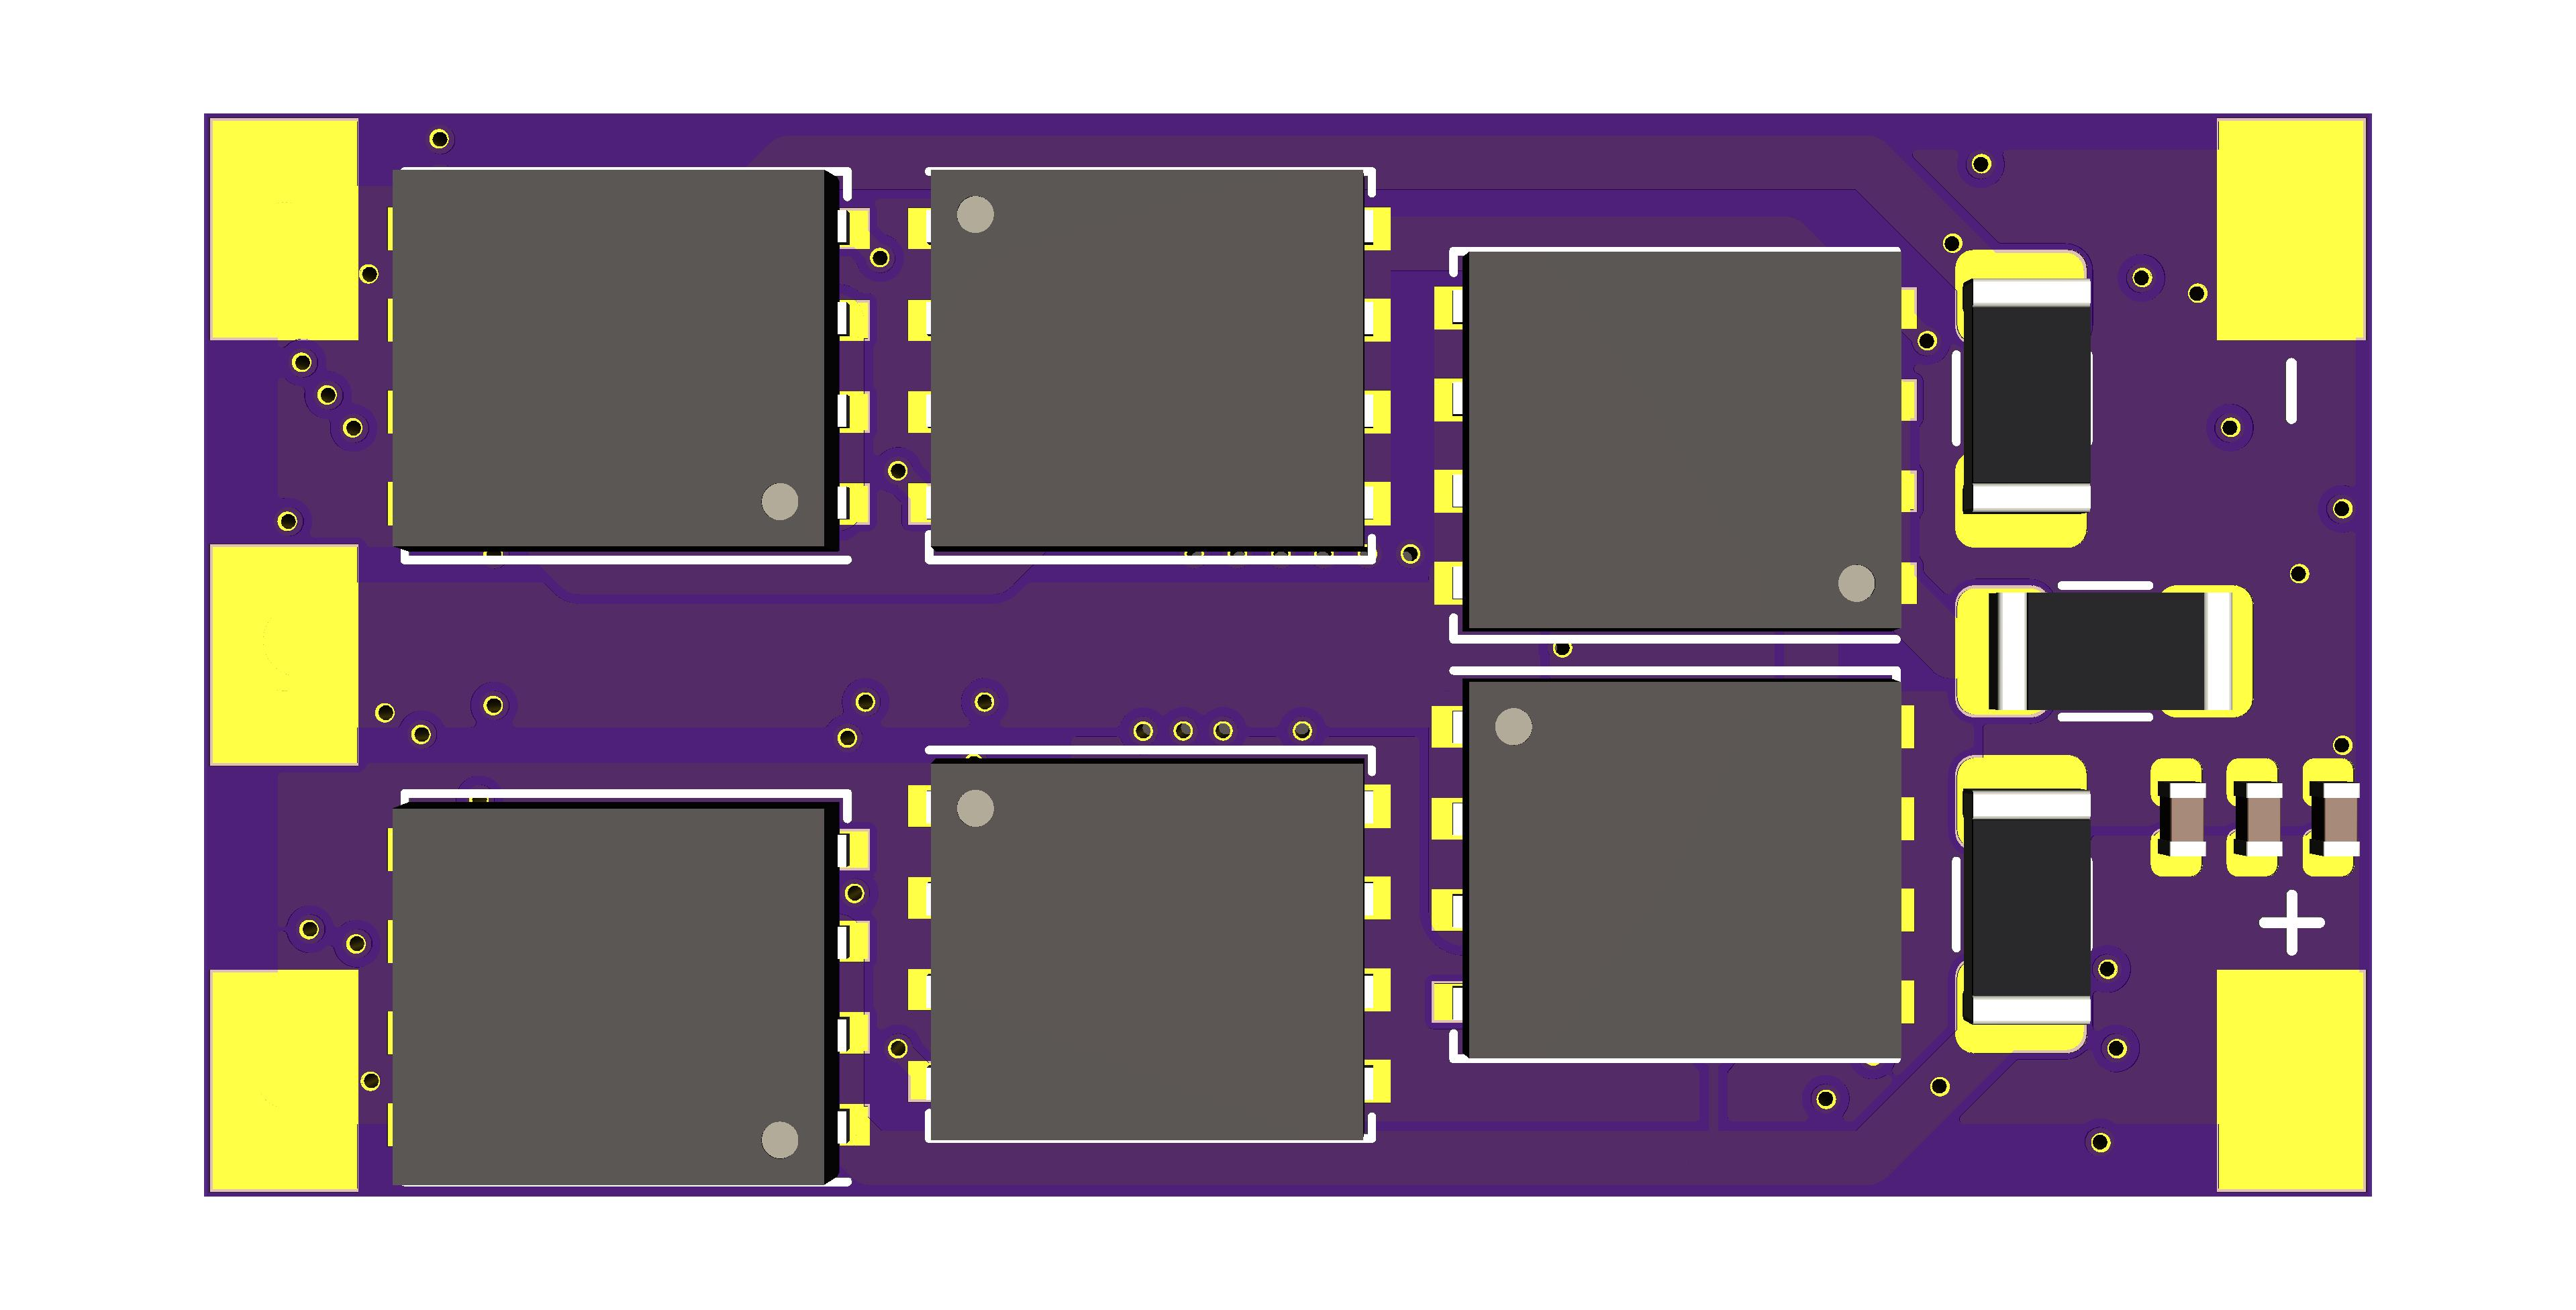
\includegraphics[width=\textwidth]{esc_back}}
	\end{center}
\end{frame}
\begin{frame}\frametitle{Project Introduction -- Primary Specifications}
	\begin{itemize}
		\item $\V{in}$: \qv{12}--\qv{25.2} (4S--6S Li-po battery)
		\item $\I{in}$: \qa{45} continuous, \qa{55} burst (5 seconds)
		\item DSHOT communication protocol support
		\item Size: comparable to off-the-shelf ESC (\qmm{15}$\times$\qmm{30})
		\item Out-of-box compatibility with broad range of motors
		\item High reliability: robustness against\ldots
		\begin{itemize}
			\item Voltage spikes
			\item Rapid throttle (speed command) changes
			\item Physical shock
		\end{itemize}
	\end{itemize}
\end{frame}
\begin{frame}\frametitle{Theory -- Brushless Motors}
	\begin{minipage}{0.5\textwidth}
		\begin{itemize}
			\item Rotor: permanent magnets
			\item Stator: coil windings
			\item Electronically commutated
			\item PMSM: sinusoidal BEMF
			\item BLDC: trapezoidal BEMF\ldots \\
			but often looks sinusoidal due to LC filtering by windings
		\end{itemize}
	\end{minipage}%
	\begin{minipage}{0.5\textwidth}
		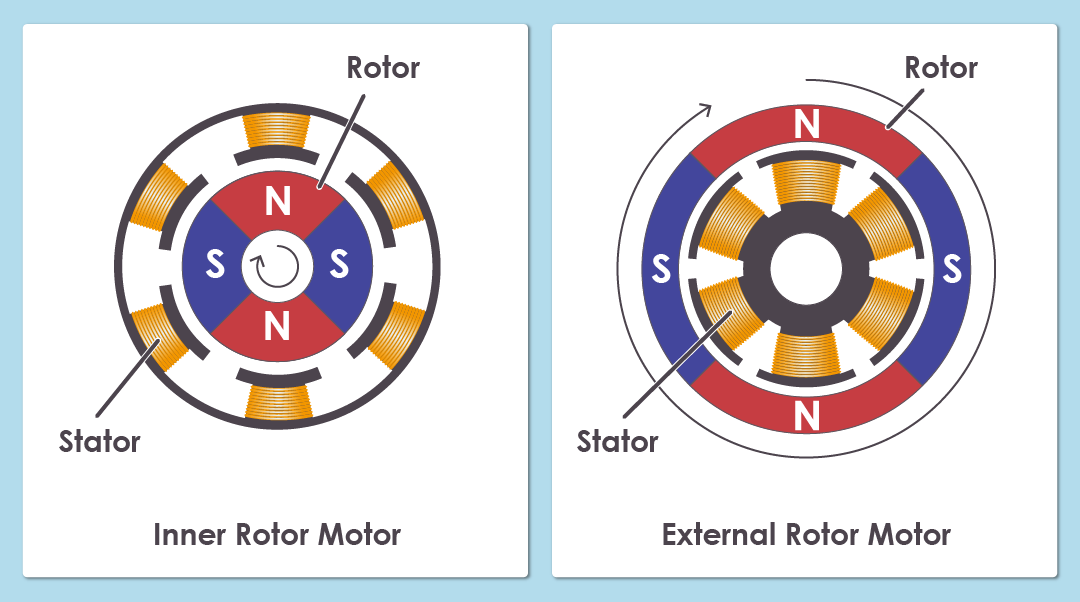
\includegraphics[width=\textwidth]{brushless_motors}
		{\scriptsize ablic.com}
		\begin{center}
			\begin{circuitikz}
	\coordinate (C) at (0,0);
	\coordinate (M) at (90:2);
	\coordinate (N) at (-30:2);
	\coordinate (P) at (210:2);
	% Inductors with filled center node and open end nodes
	\draw [L,o-*] (M) to (C);
	\draw (C) to[L,-o] (N);
	\draw [L,o-] (P) to (C);
	% Labels
	\node[above]       at (M) {U};
	\node[below right] at (N) {W};
	\node[below left]  at (P) {V};
\end{circuitikz}
		\end{center}
	\end{minipage}
\end{frame}
\begin{frame}\frametitle{Theory -- 6-Step Drive}
	\begin{minipage}{0.6\textwidth}
		Operation:
		\begin{itemize}
			\item 6 energized states
			\item Switch upon zero-crossing
			\item PWM controls torque
		\end{itemize}
		Benefits:
		\begin{itemize}
			\item Simple
			\item Low switching loss
			\item Zero-crossings measured on floating phase
		\end{itemize}
		Drawbacks:
		\begin{itemize}
			\item Torque ripple
			\item High-frequency harmonics
			\item Field not always orthogonal to rotor\ldots inefficient
		\end{itemize}
	\end{minipage}%
	\begin{minipage}{0.4\textwidth}
		\begin{center}
			\begin{tabular}{c|c c c}
	\hline
	Step & U & V & W \\
	\hline
	1 & 1 & 0 & Z \\
	2 & 1 & Z & 0 \\
	3 & Z & 1 & 0 \\
	4 & 0 & 1 & Z \\
	5 & 0 & Z & 1 \\
	6 & Z & 0 & 1 \\
	\hline
\end{tabular}
			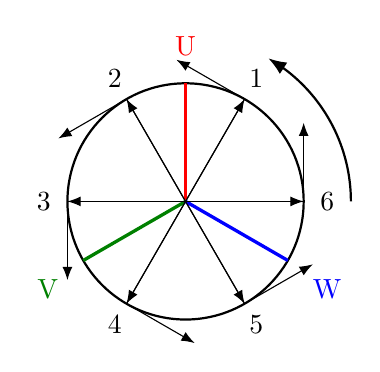
\begin{tikzpicture}[scale=0.5, >=Latex]
	\def\R{3}        % circle radius
	\def\arrlen{2.0} % tangent arrow length
	\def\n{6}        % number of tangent arrows (must be even)
	\def\rot{30}     % rotate phase axes CCW
	
	% Circle
	\draw[thick] (0,0) circle (\R);
	
	% --- Rotated phase axes (no color), label ends with x ---
	\foreach \ang/\labela/\labelb in {90+\rot/2/5, 210+\rot/4/1, 330+\rot/6/3}{
		\draw (0,0) -- ({\R*cos(\ang)},{\R*sin(\ang)});
		\draw (0,0) -- ({-\R*cos(\ang)},{-\R*sin(\ang)});
		\node at ({1.2*\R*cos(\ang)},{1.2*\R*sin(\ang)}) {$\labela$};
		\node at ({-1.2*\R*cos(\ang)},{-1.2*\R*sin(\ang)}) {$\labelb$};
	}
	
	% --- Fixed reference lines at 90°, 210°, 330° labeled U, V, W ---
	\foreach \ang/\name/\pos/\clr in {90/U/above/Red, 210/V/below left/Green, 330/W/below right/blue}{
		\draw[very thick,\clr] (0,0) -- ({\R*cos(\ang)},{\R*sin(\ang)});
		\node[\pos] at ({1.15*\R*cos(\ang)},{1.15*\R*sin(\ang)}) {\textcolor{\clr}{\name}};
	}
	
	% --- Tangent arrows (keep +30° base; rotate by \rot) ---
	% tangent at angle θ is (-sin θ, cos θ)
	\pgfmathtruncatemacro{\nm}{\n-1}
	\foreach \k in {0,...,\nm}{
		\pgfmathsetmacro{\ang}{30+\rot + 360/\n*\k}
		\pgfmathsetmacro{\px}{\R*cos(\ang)}
		\pgfmathsetmacro{\py}{\R*sin(\ang)}
		\pgfmathsetmacro{\tx}{-sin(\ang)}
		\pgfmathsetmacro{\ty}{ cos(\ang)}
		\draw[->] (\px,\py) -- ({\px+\arrlen*\tx},{\py+\arrlen*\ty});
	}
	
	% --- Diameters through opposite tangent points (same +30° base) ---
	\pgfmathtruncatemacro{\nhalf}{\n/2}
	\pgfmathtruncatemacro{\nhalfmone}{\nhalf-1}
	\foreach \k in {0,...,\nhalfmone}{
		\pgfmathsetmacro{\ang}{30+\rot + 360/\n*\k}
		\pgfmathsetmacro{\angOpp}{\ang+180}
		\pgfmathsetmacro{\px}{\R*cos(\ang)}
		\pgfmathsetmacro{\py}{\R*sin(\ang)}
		\pgfmathsetmacro{\qx}{\R*cos(\angOpp)}
		\pgfmathsetmacro{\qy}{\R*sin(\angOpp)}
		\draw[Latex-Latex] (\px,\py) -- (\qx,\qy);
	}
	
	% CCW rotation arc outside the circle
	\draw[->,thick] ({\R+1.2},0) arc[start angle=0,end angle=60,radius=\R+1.2];
\end{tikzpicture}
		\end{center}
	\end{minipage}
\end{frame}
\begin{frame}\frametitle{Theory -- Field-Oriented Control}
	\begin{minipage}{0.6\textwidth}
		Operation:
		\begin{itemize}
			\item $\infty$ energized ``states''
			\item Space-vector modulation
			\item PWM controls torque AND field orientation
		\end{itemize}
		Benefits:
		\begin{itemize}
			\item Low torque ripple
			\item Reduced harmonics
			\item Field always orthogonal to rotor\ldots highly efficient
		\end{itemize}
		Drawbacks:
		\begin{itemize}
			\item Complex
			\item Higher switching loss
			\item Difficult to measure BEMF
			\item Requires precise position sensing
		\end{itemize}
	\end{minipage}%
	\begin{minipage}{0.4\textwidth}
		\begin{center}
			\begin{tabular}{c|c c c}
	\hline
	Step & U & V & W \\
	\hline
	1 & 1 & 0 & Z \\
	2 & 1 & Z & 0 \\
	3 & Z & 1 & 0 \\
	4 & 0 & 1 & Z \\
	5 & 0 & Z & 1 \\
	6 & Z & 0 & 1 \\
	\hline
\end{tabular}
			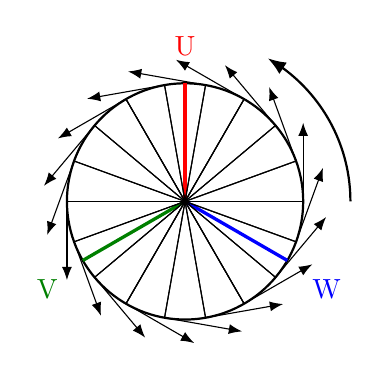
\begin{tikzpicture}[scale=0.5, >=Latex]
	\def\R{3}        % circle radius
	\def\arrlen{2} % SHORTER tangent arrow length
	\def\n{18}       % number of evenly spaced lines (must be even)
	\def\rot{30}     % rotate phase axes CCW
	
	% Circle
	\draw[thick] (0,0) circle (\R);
	
	% --- Rotated phase axes (no labels) ---
	\foreach \ang in {90+\rot, 210+\rot, 330+\rot}{
		\draw (0,0) -- ({\R*cos(\ang)},{\R*sin(\ang)});
		\draw (0,0) -- ({-\R*cos(\ang)},{-\R*sin(\ang)});
	}
	
	% --- Fixed reference lines at 90°, 210°, 330° labeled U, V, W ---
	\foreach \ang/\name/\pos/\clr in {90/U/above/Red, 210/V/below left/Green, 330/W/below right/blue}{
		\draw[very thick,\clr] (0,0) -- ({\R*cos(\ang)},{\R*sin(\ang)});
		\node[\pos] at ({1.15*\R*cos(\ang)},{1.15*\R*sin(\ang)}) {\textcolor{\clr}{\name}};
	}
	
	% --- 18 evenly spaced diameters with tangent arrows at each ---
	% Use the same +30° base so orientation stays consistent with prior figure
	\pgfmathtruncatemacro{\nm}{\n-1}
	\foreach \k in {0,...,\nm}{
		\pgfmathsetmacro{\ang}{30+\rot + 360/\n*\k}
		\pgfmathsetmacro{\angOpp}{\ang+180}
		
		% Endpoints for this diameter
		\pgfmathsetmacro{\px}{\R*cos(\ang)}
		\pgfmathsetmacro{\py}{\R*sin(\ang)}
		\pgfmathsetmacro{\qx}{\R*cos(\angOpp)}
		\pgfmathsetmacro{\qy}{\R*sin(\angOpp)}
		
		% The diameter (no labels)
		\draw (\px,\py) -- (\qx,\qy);
		
		% Tangent direction at angle ang: (-sin ang, cos ang)
		\pgfmathsetmacro{\tx}{-sin(\ang)}
		\pgfmathsetmacro{\ty}{ cos(\ang)}
		
		% Shorter tangential torque vector at the +ang endpoint
		\draw[->] (\px,\py) -- ({\px+\arrlen*\tx},{\py+\arrlen*\ty});
	}
	
	% CCW rotation arc outside the circle
	\draw[->,thick] ({\R+1.2},0) arc[start angle=0,end angle=60,radius=\R+1.2];
\end{tikzpicture}
		\end{center}
	\end{minipage}
\end{frame}
\begin{frame}\frametitle{Theory -- Clarke-Park Transforms}
	\begin{center}
		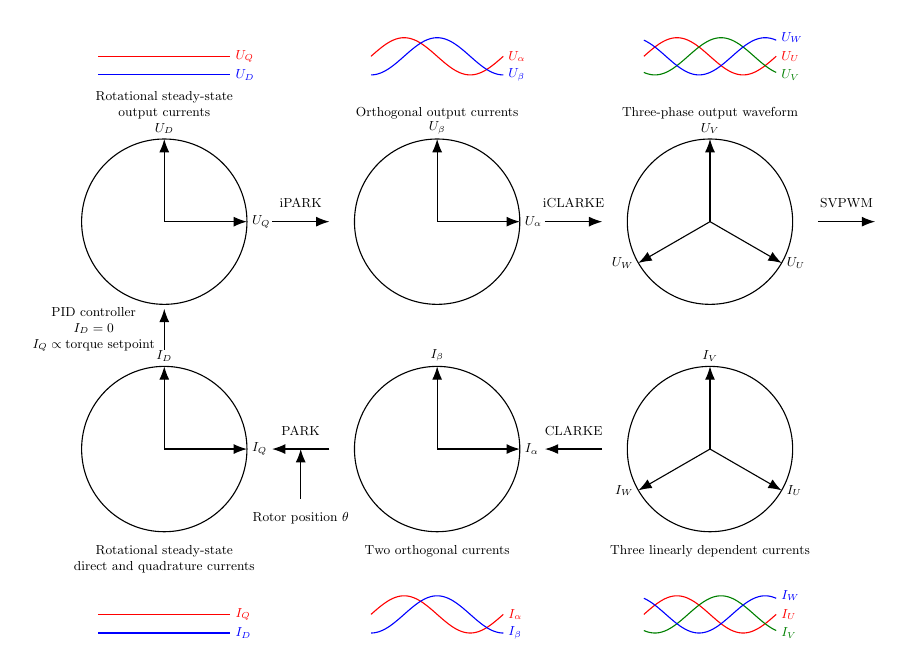
\begin{tikzpicture}[scale=0.525, every node/.style={transform shape}, >=Latex]
	% --- knobs ---
	\def\R{2}        % circle radius (cm)
	\def\W{3.2}      % waveform width
	\def\A{0.45}     % waveform amplitude
	\def\wfpadT{2} % padding above top circles
	\def\wfpadB{2} % padding below bottom circles
	
	% --- styles ---
	\tikzset{
		circ/.style = {draw, circle, minimum size=2*\R cm},
		axis/.style = {-Latex},
		vec/.style  = {-Latex},
		lbl/.style  = {font=\small}
	}
	
	% --- layout anchors ---
	\coordinate (T1) at (0,5.5);
	\coordinate (T2) at (6.6,5.5);
	\coordinate (T3) at (13.2,5.5);
	\coordinate (B1) at (0,0);
	\coordinate (B2) at (6.6,0);
	\coordinate (B3) at (13.2,0);
	
	% ================== TOP ROW — VOLTAGE ==================
	\node[circ] (C_T1) at (T1) {};
	\draw[axis] (C_T1.center) -- ++(0,\R) node[lbl,above] {$U_D$};
	\draw[axis] (C_T1.center) -- ++(\R,0) node[lbl,right] {$U_Q$};
	\node[align=center, lbl, above=10pt of C_T1] {Rotational steady-state \\ output currents};
	
	\node[circ] (C_T2) at (T2) {};
	\draw[axis] (C_T2.center) -- ++(0,\R) node[lbl,above] {$U_\beta$};
	\draw[axis] (C_T2.center) -- ++(\R,0) node[lbl,right] {$U_\alpha$};
	\node[align=center, lbl, above=10pt of C_T2] {Orthogonal output currents};
	
	\node[circ] (C_T3) at (T3) {};
	\foreach \ang/\name/\pos in {90/U_V/above, -30/U_U/right, -150/U_W/left}{
		\draw[vec] (C_T3.center) -- ++(\ang:\R);
		\node[lbl,\pos] at ($(C_T3.center)+(\ang:\R)$) {$\name$};
	}
	\node[align=center, lbl, above=10pt of C_T3] {Three-phase output waveform};
	
	% arrows across the top row
	\draw[-Latex] ($(C_T1.east)+(0.6,0)$) -- node[above=6pt,lbl]{iPARK}    ($(C_T2.west)+(-0.6,0)$);
	\draw[-Latex] ($(C_T2.east)+(0.6,0)$) -- node[above=6pt,lbl]{iCLARKE} ($(C_T3.west)+(-0.6,0)$);
	\draw[-Latex] ($(C_T3.east)+(0.6,0)$) -- node[above=6pt,lbl]{SVPWM} ($(C_T3.east)+(0.6,0)+(C_T3.west)+(-0.6,0)-(C_T2.east)-(0.6,0)$);
	
	% ================== BOTTOM ROW — CURRENT ==================
	\node[circ] (C_B1) at (B1) {};
	\draw[axis] (C_B1.center) -- ++(0,\R) node[lbl,above] {$I_D$};
	\draw[axis] (C_B1.center) -- ++(\R,0) node[lbl,right] {$I_Q$};
	\node[align=center, lbl, below=6pt of C_B1] {Rotational steady-state \\ direct and quadrature currents};
	
	\node[circ] (C_B2) at (B2) {};
	\draw[axis] (C_B2.center) -- ++(0,\R) node[lbl,above] {$I_\beta$};
	\draw[axis] (C_B2.center) -- ++(\R,0) node[lbl,right] {$I_\alpha$};
	\node[align=center, lbl, below=6pt of C_B2] {Two orthogonal currents};
	
	\node[circ] (C_B3) at (B3) {};
	\foreach \ang/\name/\pos in {90/I_V/above, -30/I_U/right, -150/I_W/left}{
		\draw[vec] (C_B3.center) -- ++(\ang:\R);
		\node[lbl,\pos] at ($(C_B3.center)+(\ang:\R)$) {$\name$};
	}
	\node[align=center, lbl, below=6pt of C_B3] {Three linearly dependent currents};
	
	% arrows across the bottom row
	\draw[-Latex] ($(C_B3.west)+(-0.6,0)$) -- node[above=6pt,lbl]{CLARKE} ($(C_B2.east)+(0.6,0)$);
	\draw[-Latex] ($(C_B2.west)+(-0.6,0)$) -- node[above=6pt,lbl]{PARK}  ($(C_B1.east)+(0.6,0)$);
	\draw[-Latex] ($(C_B1.east)!0.5!(C_B2.west)-(0,1.2)$) node[below=6pt,lbl]{Rotor position $\theta$} -- ($(C_B1.east)!0.5!(C_B2.west)$);
	
	% PID controllers arrow (downward)
	\draw[Latex-]
	($(C_T1.south)+(0,-0.1)$) -- node[lbl,left=3pt,align=center]{PID controller\\$I_{D}=0$\\$I_{Q}\propto\text{torque setpoint}$}
	($(C_B1.north)+(0,0.4)$);
	
	% ================== WAVEFORMS ==================
	% ---- TOP: above circles ----
	\begin{scope}[shift={($(C_T1.center)+(0,\R+\wfpadT)$)}]
		\draw [Red] ({-0.5*\W},0) -- ({0.5*\W},0)
		node[Red,lbl,anchor=west] {$U_Q$};
		\draw [blue] ({-0.5*\W},-\A) -- ({0.5*\W},-\A)
		node[blue,lbl,anchor=west] {$U_D$};
	\end{scope}
	
	\begin{scope}[shift={($(C_T2.center)+(0,\R+\wfpadT)$)}]
		\draw[Red,samples=120,domain=0:360,variable=\t,smooth]
		plot ({-0.5*\W + \W*\t/360},{ \A*sin(\t)}) node[Red,lbl,anchor=west] at ({0.5*\W},{0}) {$U_\alpha$};
		\draw[blue,samples=120,domain=0:360,variable=\t,smooth]
		plot ({-0.5*\W + \W*\t/360},{ \A*sin(\t-90)}) node[blue,lbl,anchor=west] at ({0.5*\W},{-\A}) {$U_\beta$};
	\end{scope}
	
	\begin{scope}[shift={($(C_T3.center)+(0,\R+\wfpadT)$)}]
		\draw[Red,samples=120,domain=0:360,variable=\t,smooth]
		plot ({-0.5*\W + \W*\t/360},{ \A*sin(\t)}) node[Red,lbl,anchor=west] at ({0.5*\W},{0}) {$U_U$};
		\draw[Green,samples=120,domain=0:360,variable=\t,smooth]
		plot ({-0.5*\W + \W*\t/360},{ \A*sin(\t-120)}) node[Green,lbl,anchor=west] at ({0.5*\W},{-\A}) {$U_V$};
		\draw[blue,samples=120,domain=0:360,variable=\t,smooth]
		plot ({-0.5*\W + \W*\t/360},{ \A*sin(\t+120)}) node[blue,lbl,anchor=west] at ({0.5*\W},{\A}) {$U_W$};
	\end{scope}
	
	% ---- BOTTOM: below circles ----
	\begin{scope}[shift={($(C_B1.center)+(0,-\R-\wfpadB)$)}]
		\draw [Red] ({-0.5*\W},0) -- ({0.5*\W},0)
		node[Red,lbl,anchor=west] {$I_Q$};
		\draw [blue] ({-0.5*\W},-\A) -- ({0.5*\W},-\A)
		node[Blue,lbl,anchor=west] {$I_D$};
	\end{scope}
	
	\begin{scope}[shift={($(C_B2.center)+(0,-\R-\wfpadB)$)}]
		\draw[Red,samples=120,domain=0:360,variable=\t,smooth]
		plot ({-0.5*\W + \W*\t/360},{ \A*sin(\t)}) node[Red,lbl,anchor=west] at ({0.5*\W},{0}) {$I_\alpha$};
		\draw[blue,samples=120,domain=0:360,variable=\t,smooth]
		plot ({-0.5*\W + \W*\t/360},{ \A*sin(\t-90)});
		\node[blue,lbl,anchor=west] at ({0.5*\W},{-\A}) {$I_\beta$};
	\end{scope}
	
	\begin{scope}[shift={($(C_B3.center)+(0,-\R-\wfpadB)$)}]
		\draw[Red,samples=120,domain=0:360,variable=\t,smooth]
		plot ({-0.5*\W + \W*\t/360},{ \A*sin(\t)}) node[Red,lbl,anchor=west] at ({0.5*\W},{0}) {$I_U$};
		\draw[Green,samples=120,domain=0:360,variable=\t,smooth]
		plot ({-0.5*\W + \W*\t/360},{ \A*sin(\t-120)}) node[Green,lbl,anchor=west] at ({0.5*\W},{-\A}) {$I_V$};
		\draw[blue,samples=120,domain=0:360,variable=\t,smooth]
		plot ({-0.5*\W + \W*\t/360},{ \A*sin(\t+120)});
		\node[blue,lbl,anchor=west] at ({0.5*\W},{\A}) {$I_W$};
	\end{scope}
\end{tikzpicture}

	\end{center}
\end{frame}
\begin{frame}\frametitle{Theory -- Sensorless Position Estimation}
	Key point: $\text{knowing BEMF and phase currents}=\text{knowing rotor position}$
	\begin{enumerate}
		\item Measure phase voltage during short non-energized intervals
		\begin{itemize}
			\item High speed required for large BEMF\ldots
			\item but non-energized intervals shorten as speed increases
		\end{itemize}
		\item Estimate BEMF using measured currents and motor parameters $L$ and $R$ per phase
		\item Calculate electrical angle of rotor, differentiate w.r.t. time to obtain speed
		\begin{itemize}
			\item Helps to know rotor inertia
		\end{itemize}
	\end{enumerate}
	More advanced techniques: high-frequency injection, PLL, etc.
\end{frame}
\begin{frame}\frametitle{Design Walkthrough -- Schematic}
	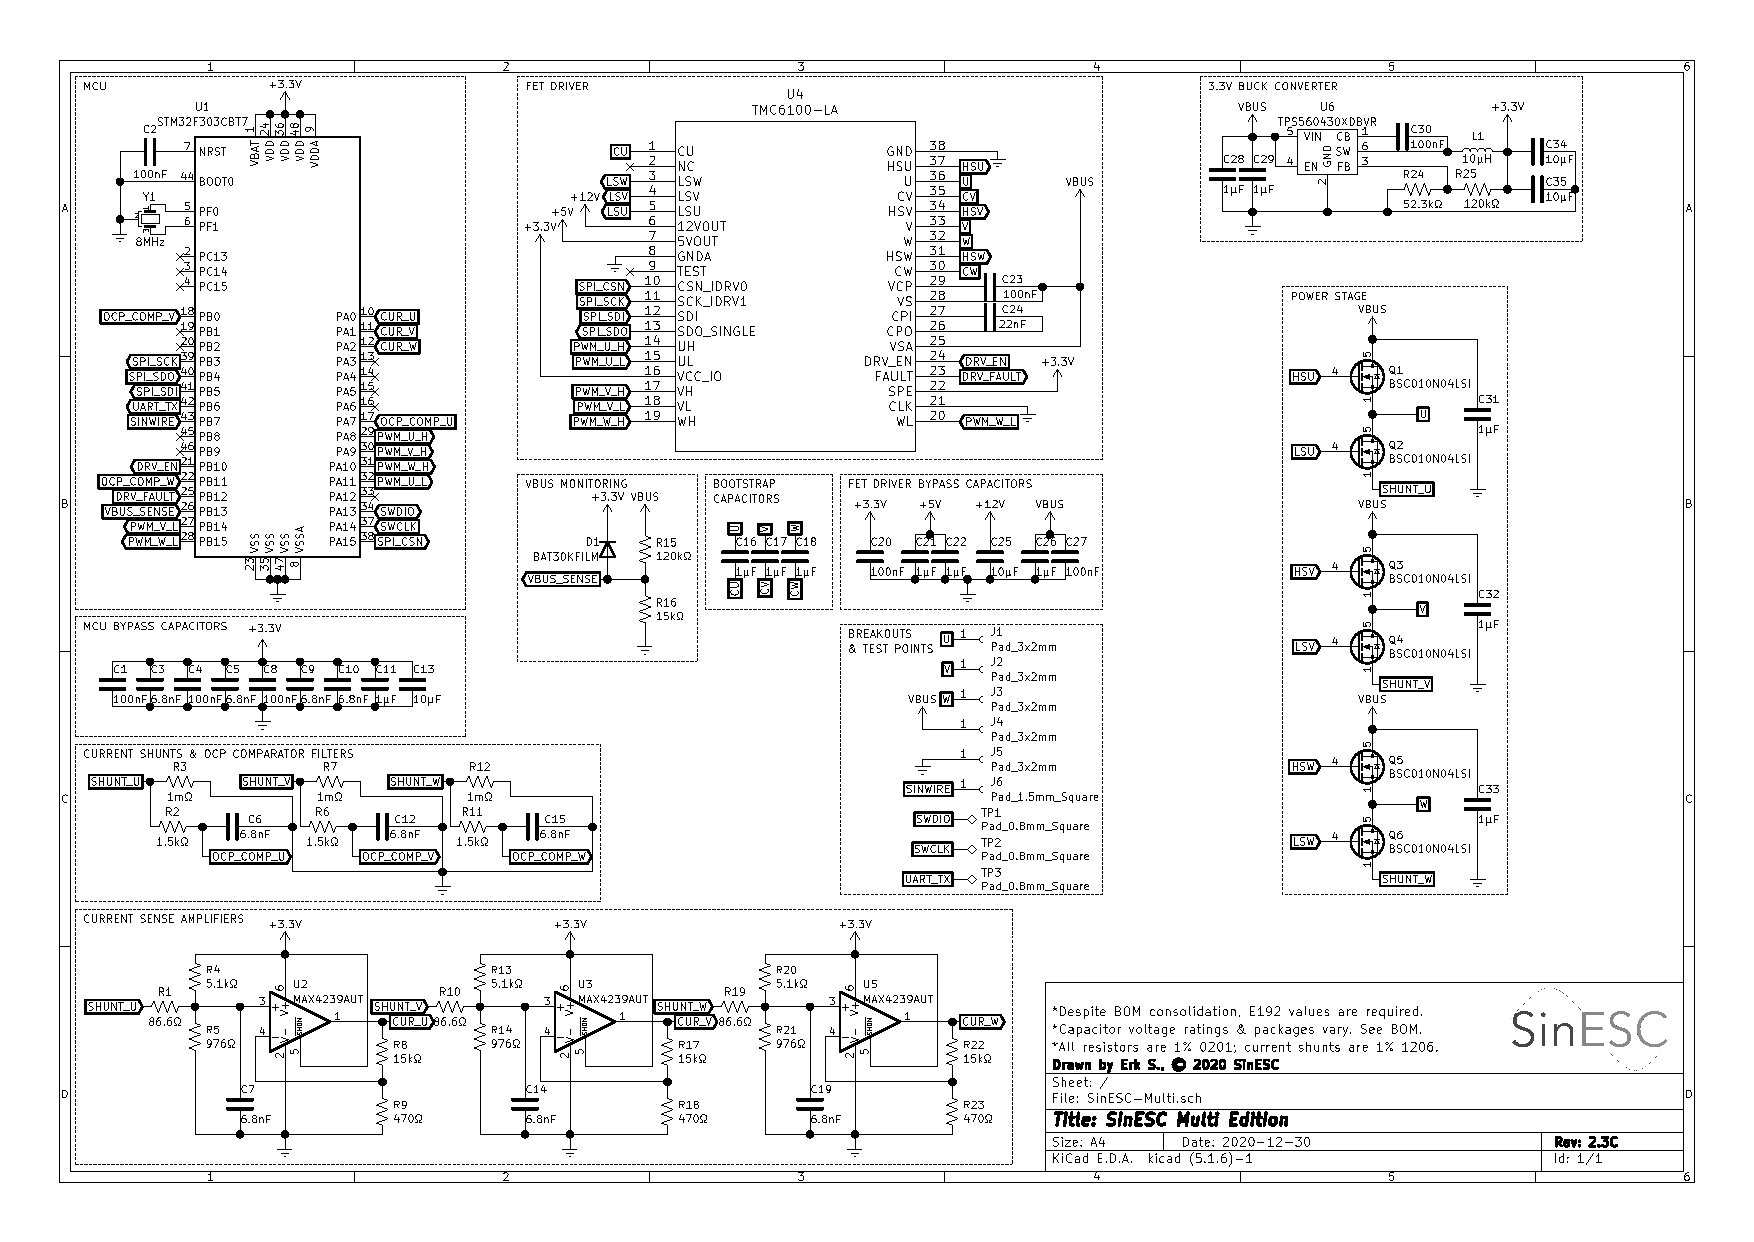
\includegraphics[width=\textwidth]{schematic}
\end{frame}
\begin{frame}\frametitle{Design Walkthrough -- Key Component Characteristics}
	\begin{minipage}[t]{0.5\textwidth}
		Microcontroller
		\begin{itemize}
			\item ST part -- FOC library
			\item Ample analog peripherals
			\item 32 bit, medium performance
		\end{itemize}
	\end{minipage}%
	\begin{minipage}[t]{0.5\textwidth}
		Current-sense amplifiers
		\begin{itemize}
			\item Low noise
			\item Sufficient bandwidth
			\item Temperature stability
		\end{itemize}
	\end{minipage}
	\vskip 1em
	\begin{minipage}[t]{0.5\textwidth}
		FET driver
		\begin{itemize}
			\item Simplicity
			\item Robustness against transients
			\item Sufficient drive current
			\item High-side N support
		\end{itemize}
	\end{minipage}%
	\begin{minipage}[t]{0.5\textwidth}
		MOSFETs
		\begin{itemize}
			\item $\R{ds,on}$ low enough
			\item $Q_{\text{g}}$ as low as possible
			\item Sufficient $\V{ds}$
			\item N-channel
		\end{itemize}
	\end{minipage}
\end{frame}
\begin{frame}\frametitle{Design Walkthrough -- Component Choices}
	\begin{minipage}[t]{0.5\textwidth}
		Microcontroller: STM32F3xx
		\begin{itemize}
			\item Multiple ADCs
			\item Comparators for OCP
			\item ST FOC library
			\item Cortex-M3
		\end{itemize}
	\end{minipage}%
	\begin{minipage}[t]{0.5\textwidth}
		Current-sense amplifiers: MAX4239
		\begin{itemize}
			\item Somewhat poor choice
			\item \quv{0.1} input offset voltage unnecessary
			\item Too expensive
		\end{itemize}
	\end{minipage}
	\vskip 1em
	\begin{minipage}[t]{0.5\textwidth}
		FET driver: TMC6100
		\begin{itemize}
			\item Expensive and complicated
			\item Charge pump for 100\% duty cycle operation
			\item Controlled through SPI
		\end{itemize}
	\end{minipage}%
	\begin{minipage}[t]{0.5\textwidth}
		MOSFETS: BSC010N04LSI
		\begin{itemize}
			\item $\V{ds}=\qv{40}$
			\item $R_{\text{ds,on}}=\qmr{1.05}$: too low
			\item $Q_{\text{g}}=\qnc{87}$: too high
			\item Ideally, find middle ground by considering product $R_{\text{ds,on}}Q_{\text{g}}$
		\end{itemize}
	\end{minipage}
\end{frame}
\begin{frame}\frametitle{Design Walkthrough -- Challenges}
	\begin{minipage}{0.6\textwidth}
		\begin{itemize}
			\item SPI configuration
			\item Inappropriate current specification
			\item \qv{3.3} rail issue
			\item Gate driver charge pump filter
			\item Form factor; difficulty with testing
			\item ADC resolution for current sensing
		\end{itemize}
	\end{minipage}%
	\begin{minipage}{0.4\textwidth}
		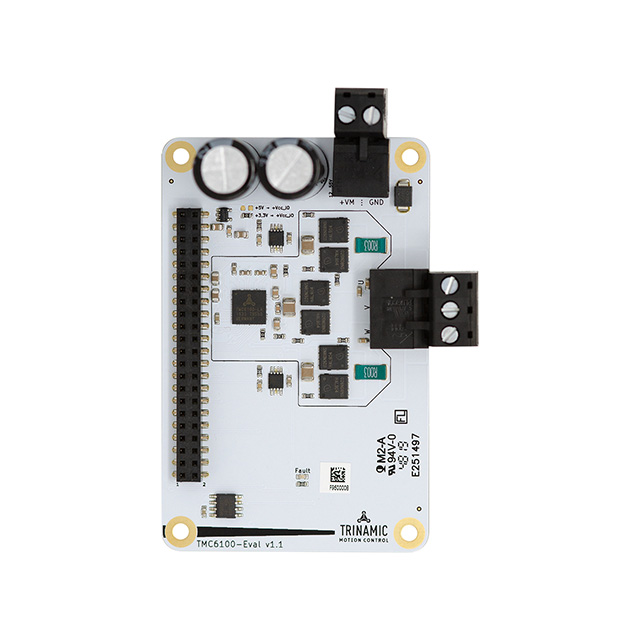
\includegraphics[width=\textwidth]{form_factor}
	\end{minipage}
	\begin{center}
		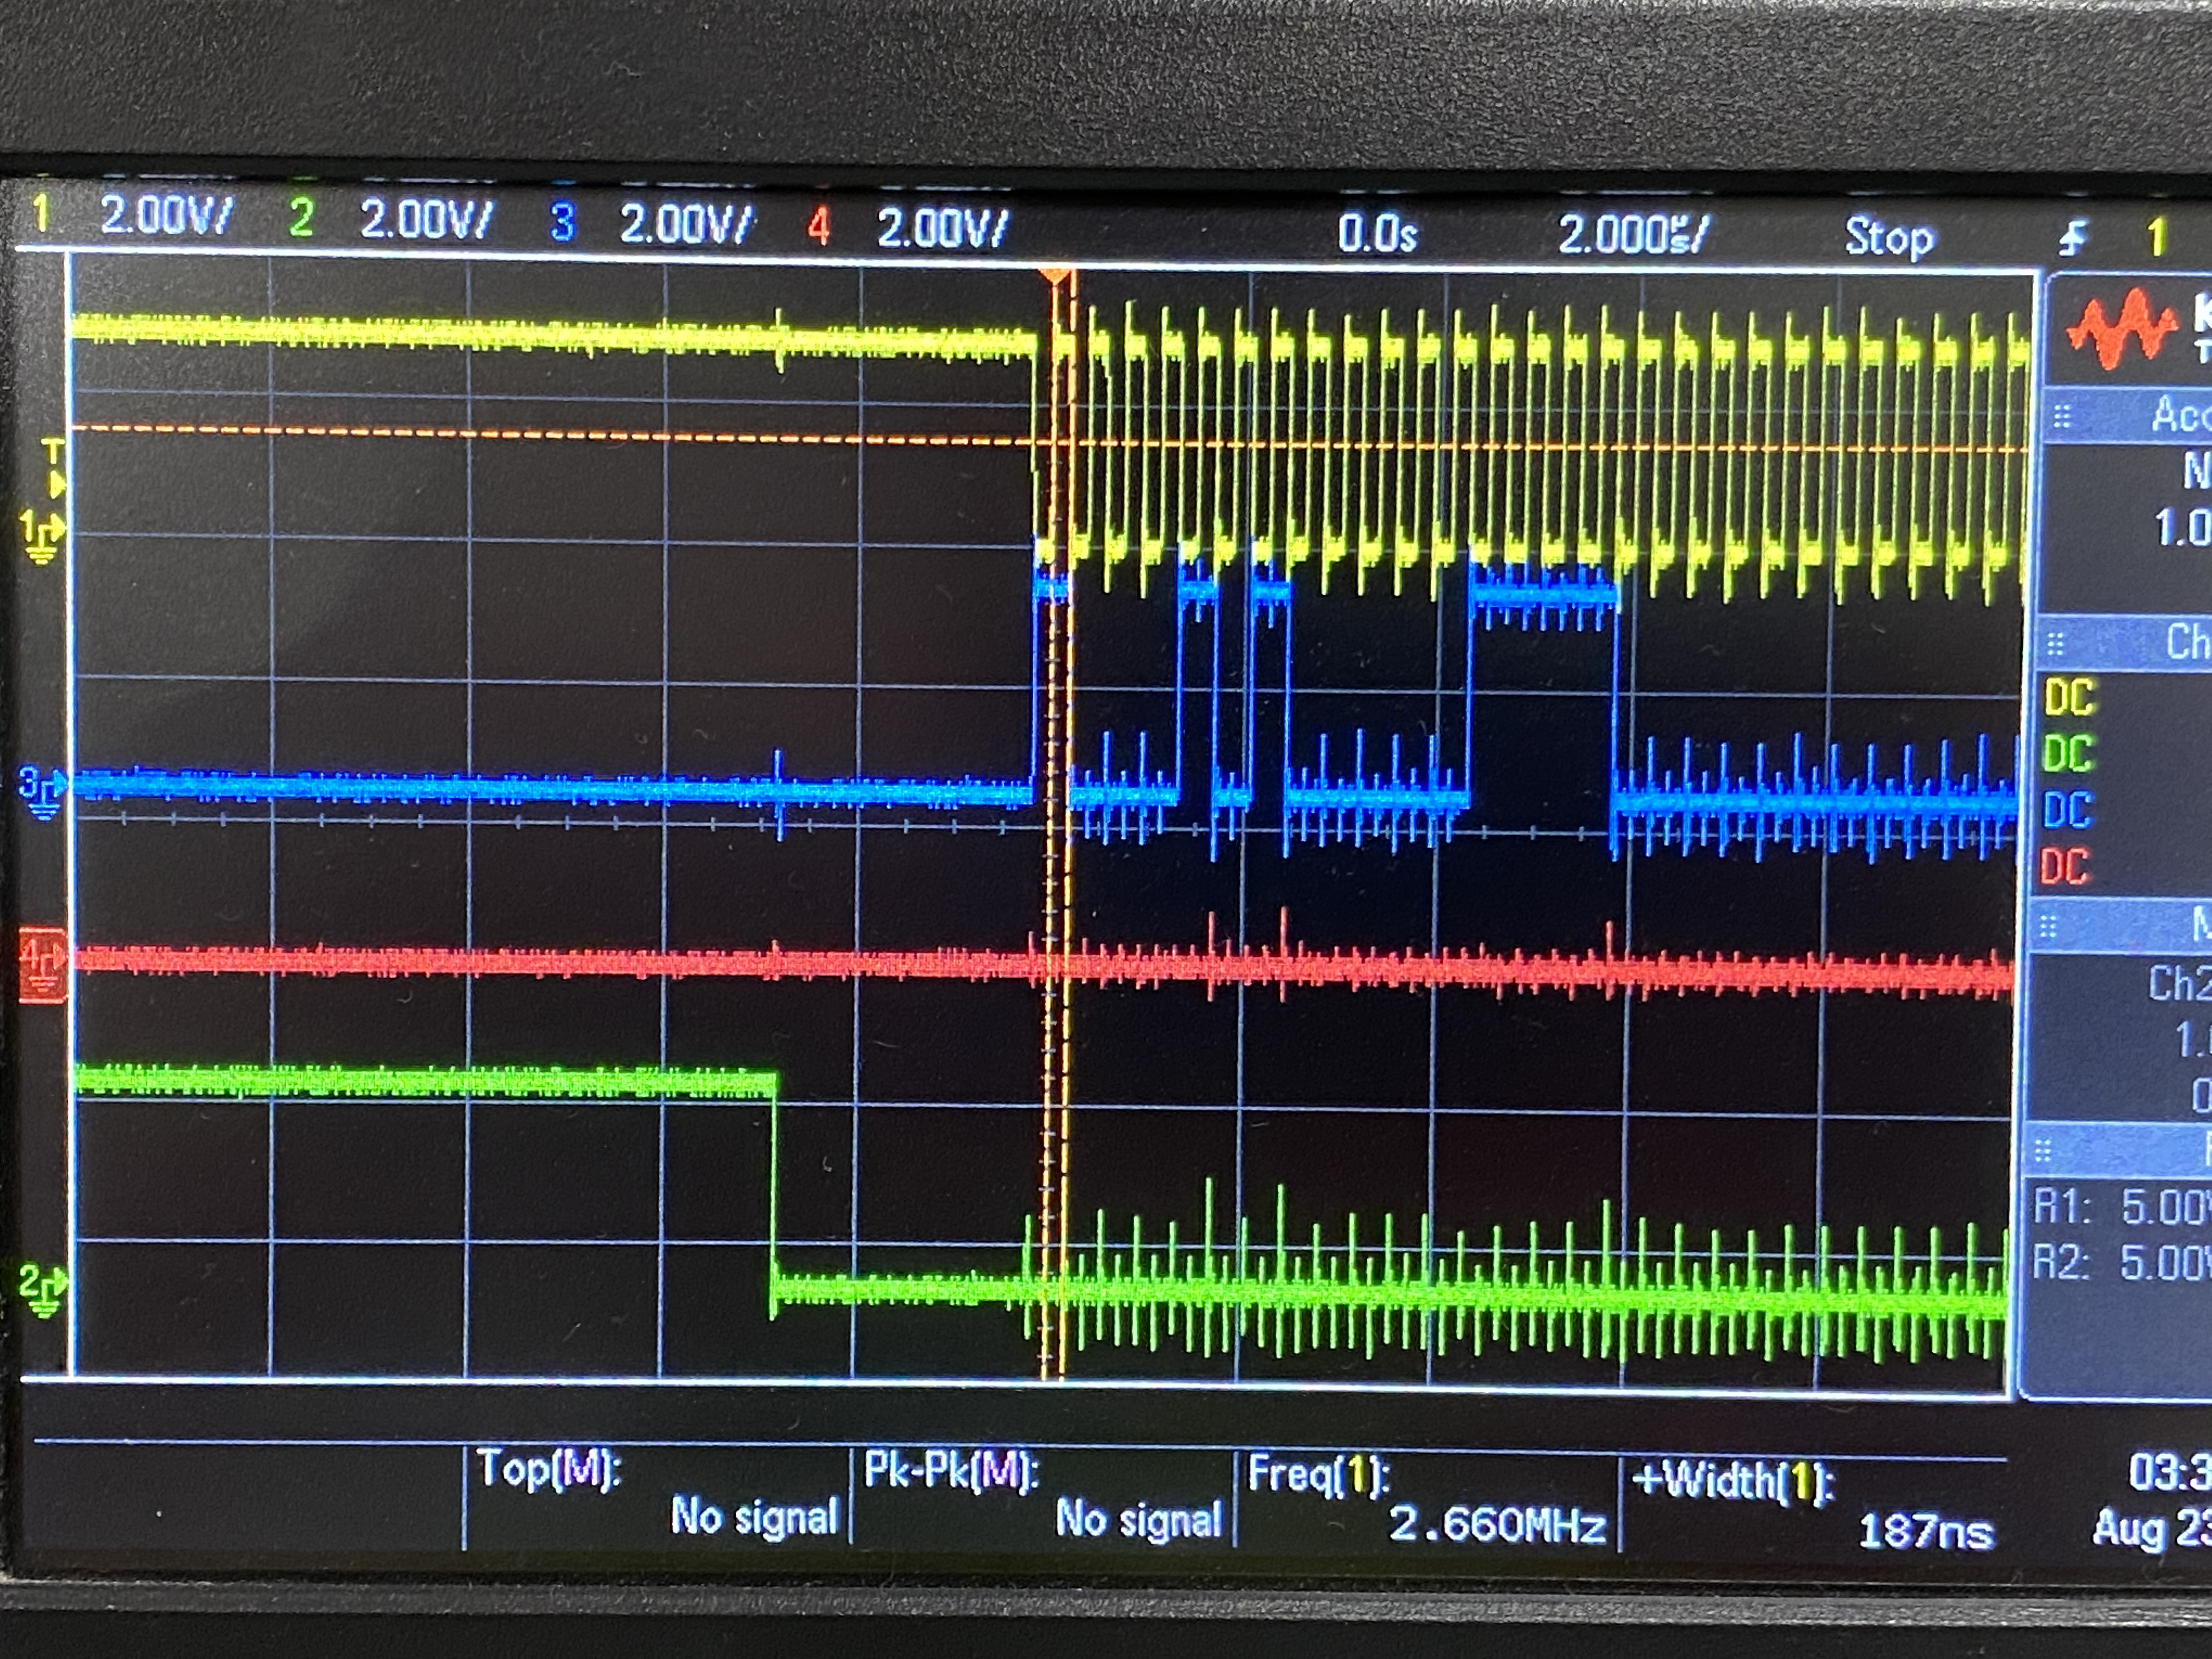
\includegraphics[width=0.45\textwidth]{spi1}
		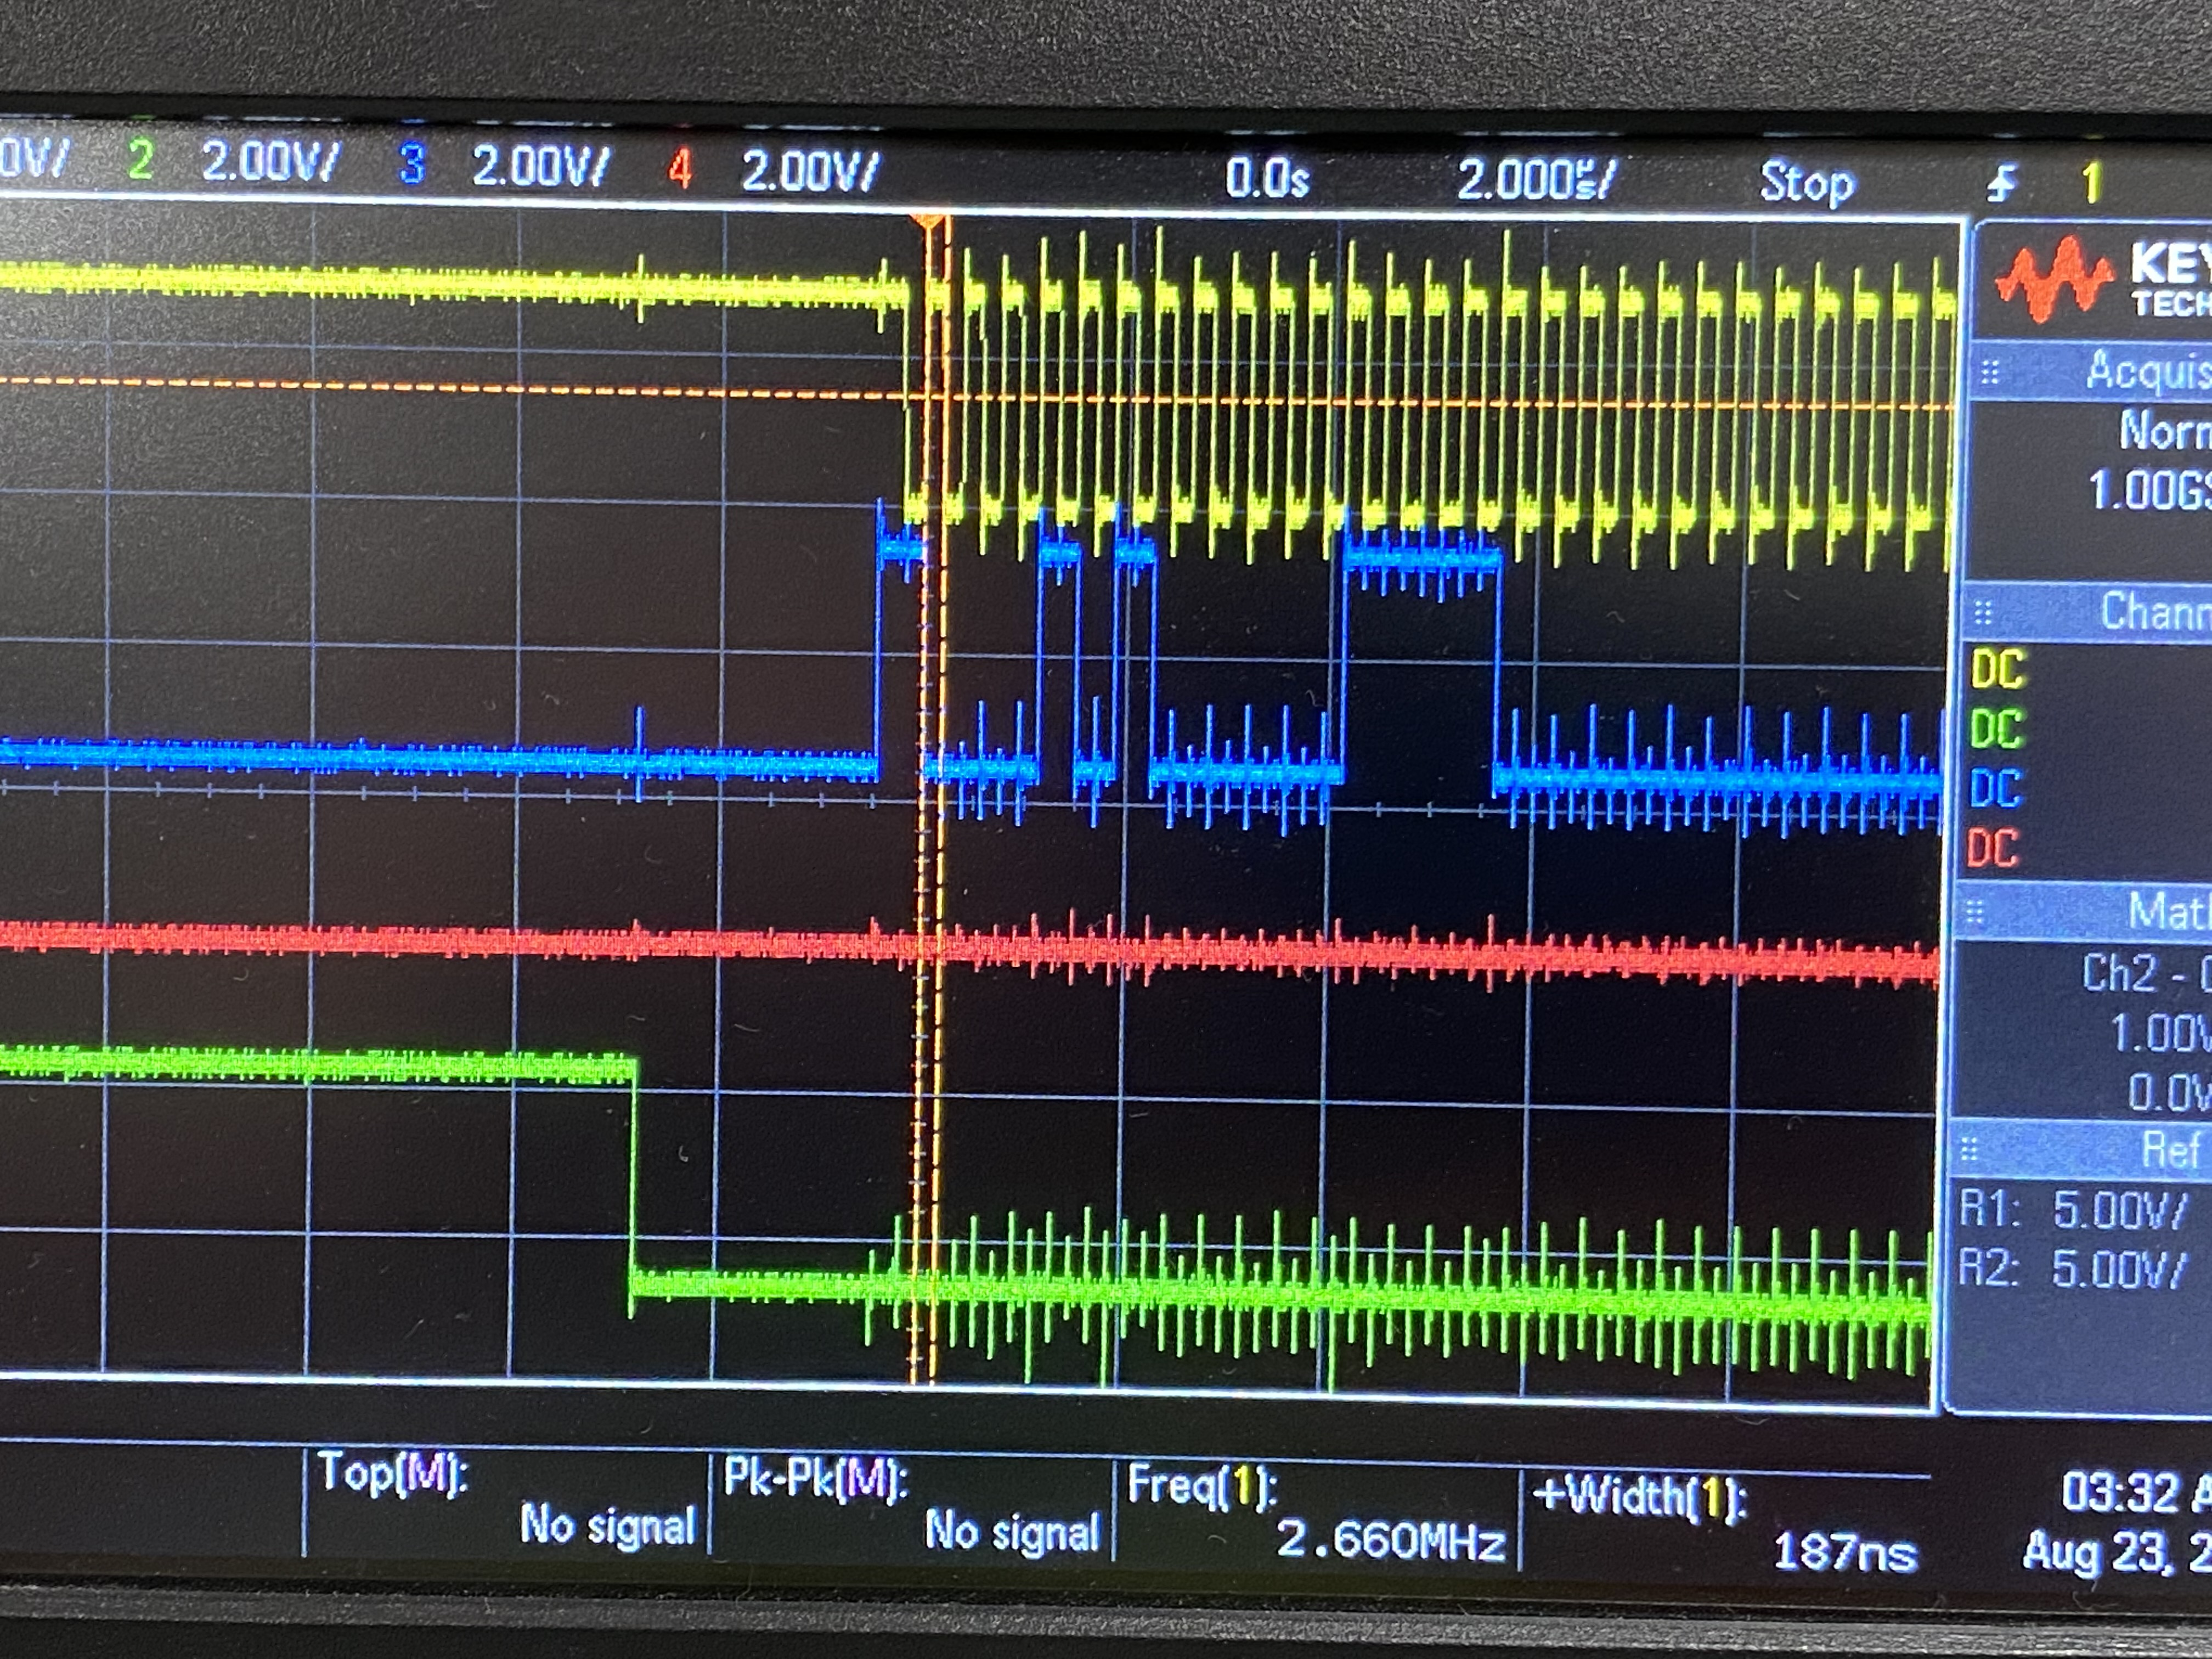
\includegraphics[width=0.45\textwidth]{spi2}
	\end{center}
\end{frame}
\begin{frame}\frametitle{Design Walkthrough -- Assembly}
	\begin{itemize}
		\item Initially: stencil, pick \& place, and reflow manually
		\item Later: assembled at PCBWay
	\end{itemize}
	\begin{center}
		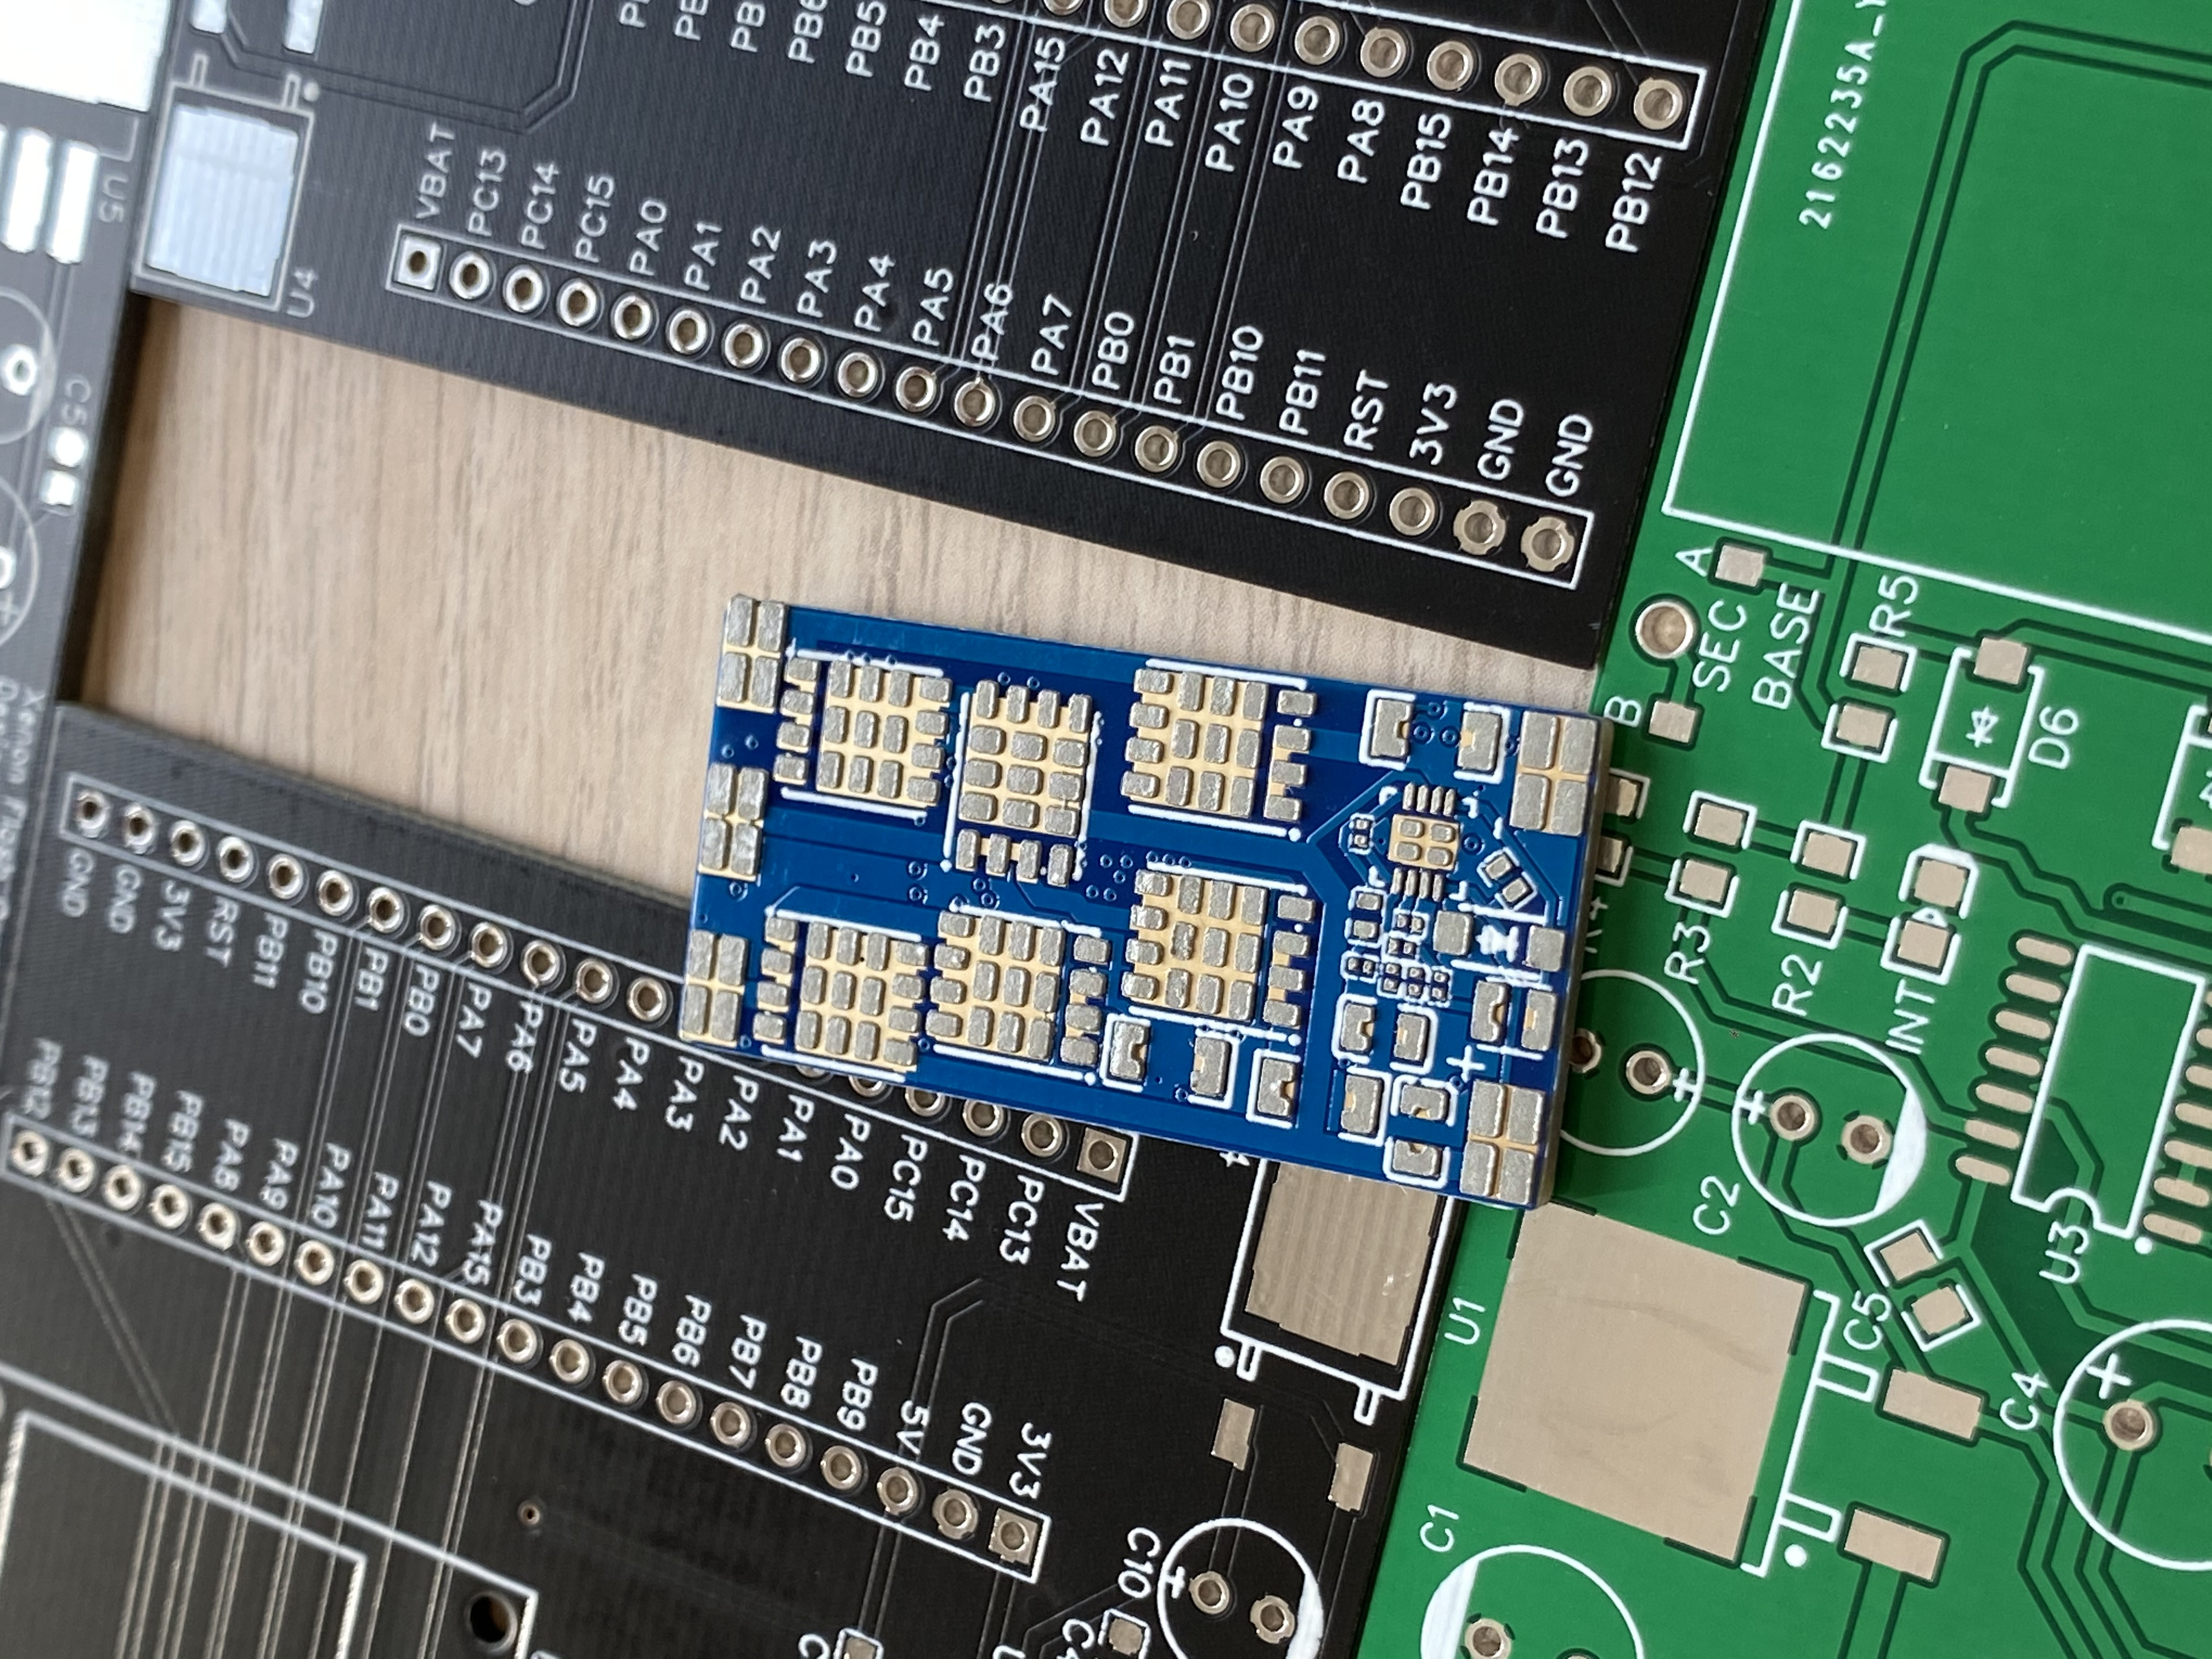
\includegraphics[width=0.45\textwidth]{stencil}
		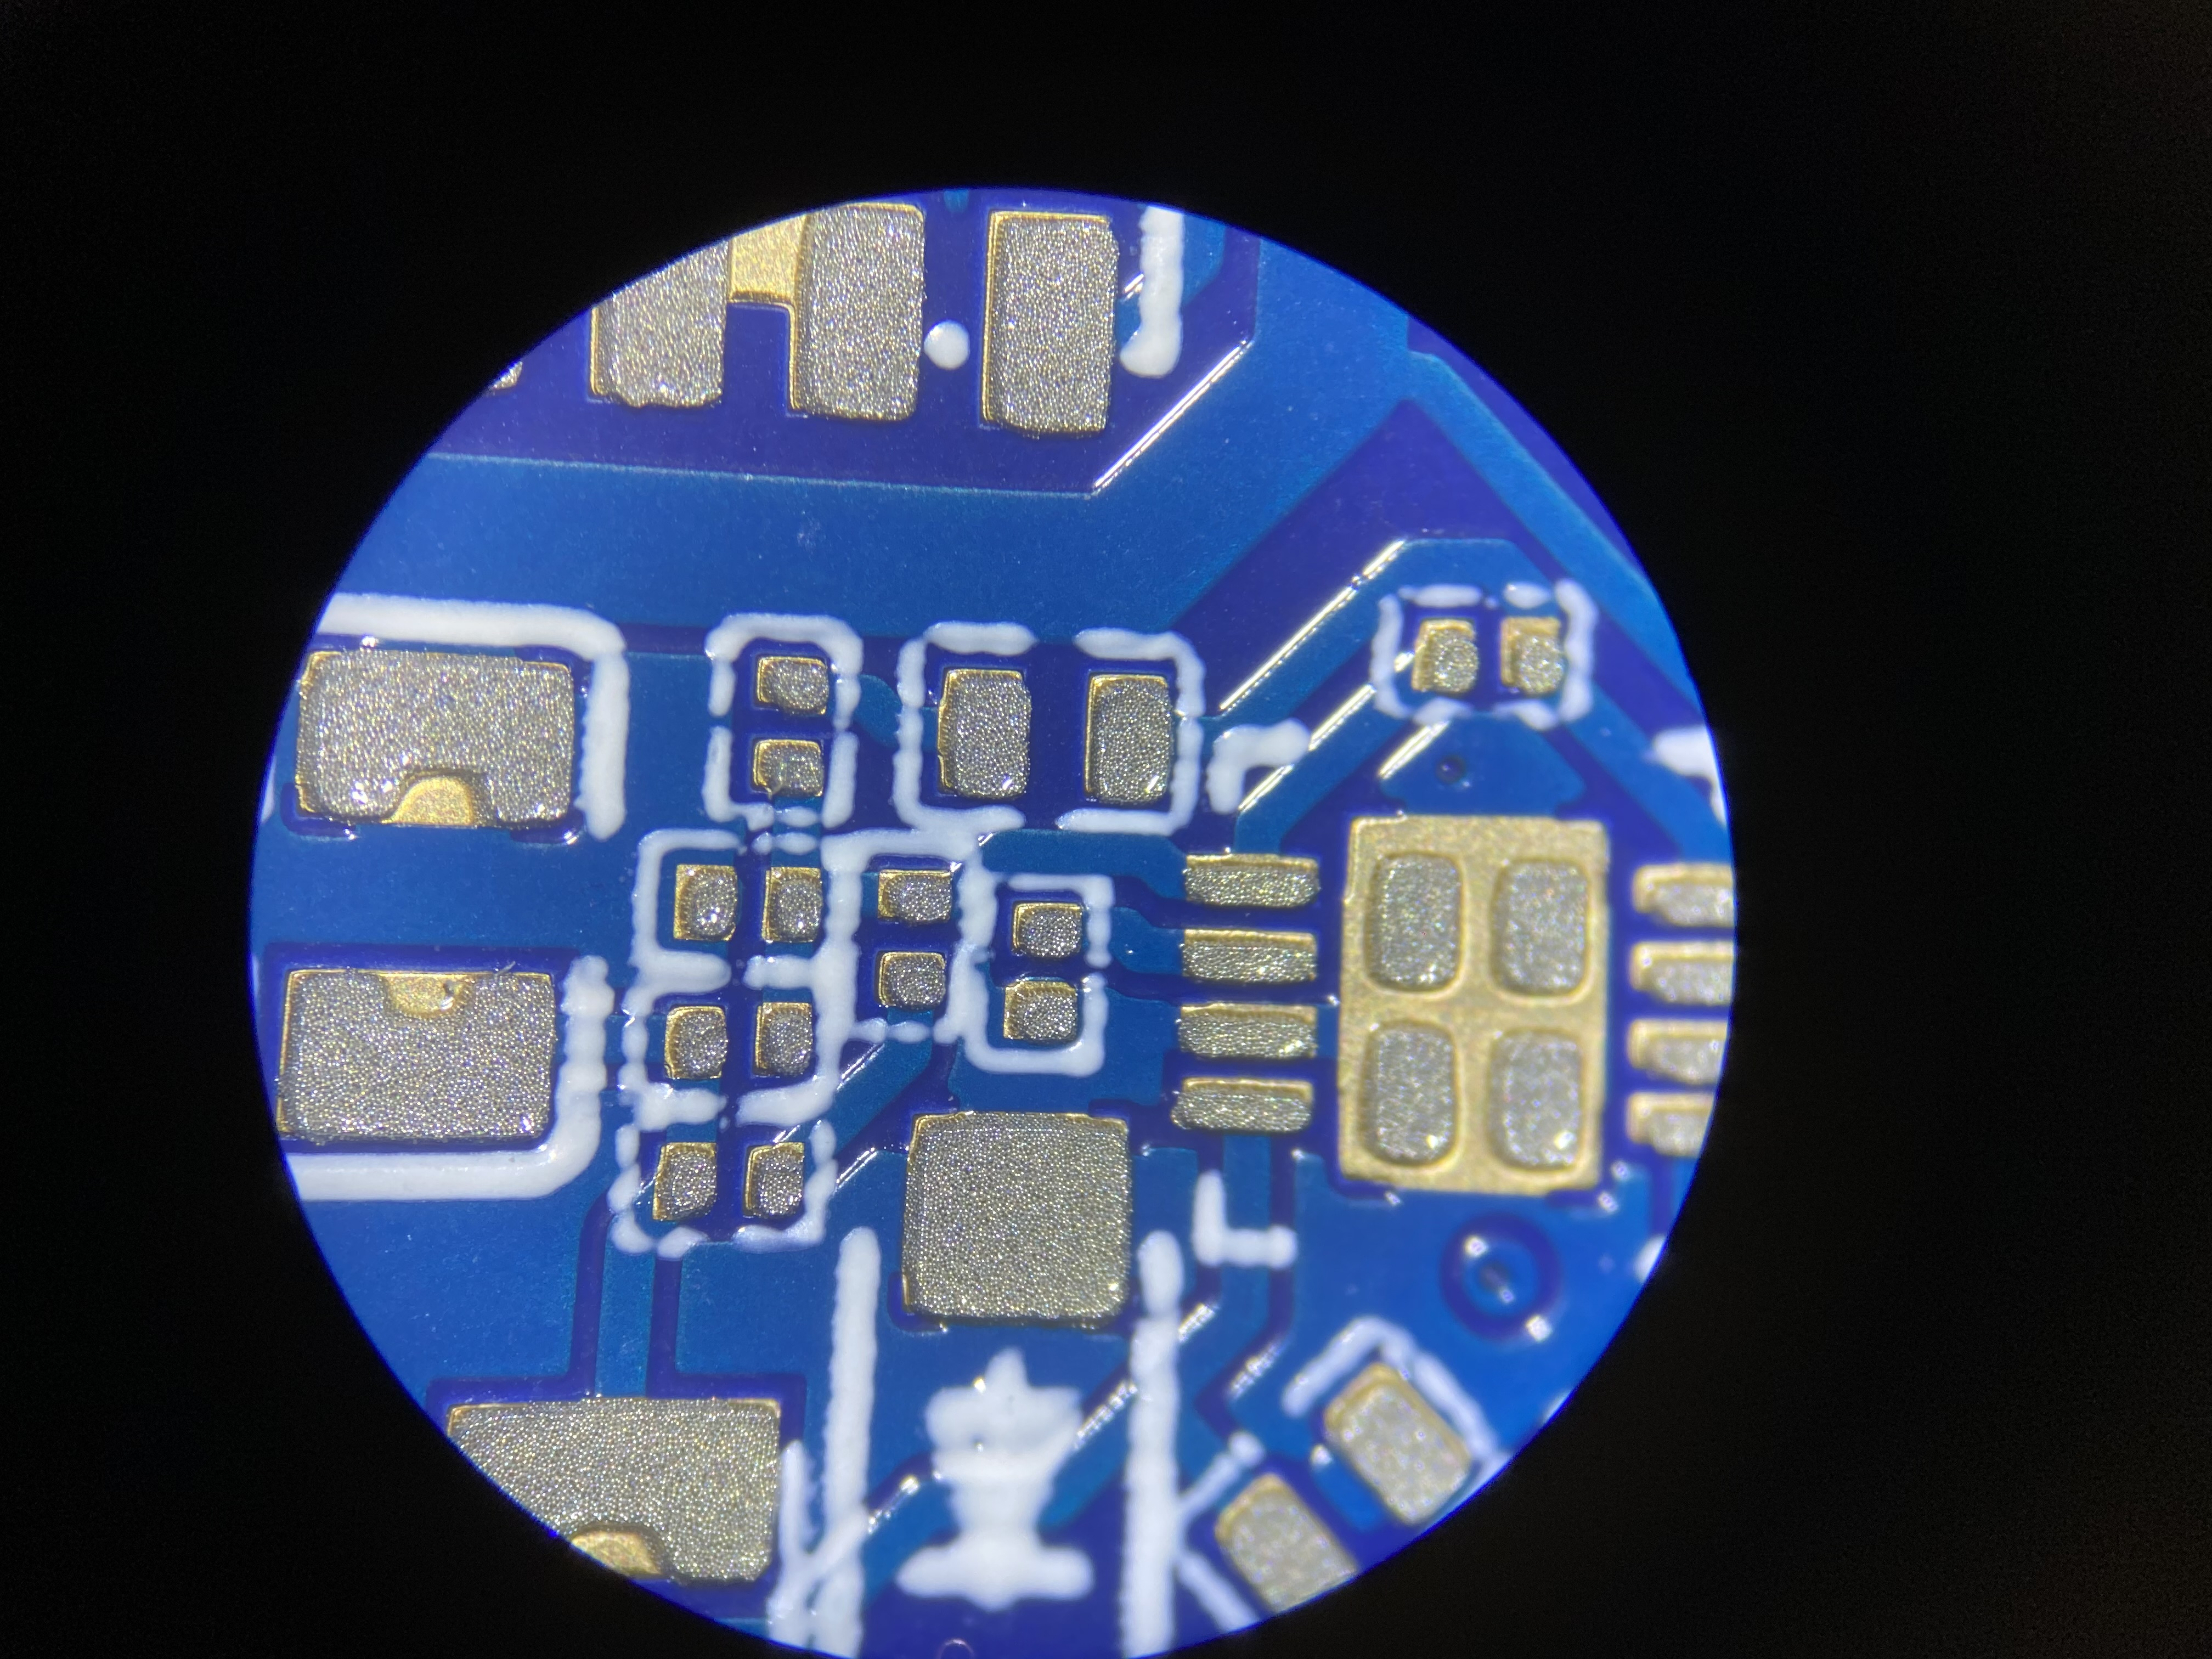
\includegraphics[width=0.45\textwidth]{stencil_microscope}
	\end{center}
\end{frame}
\end{document}